\documentclass[../notes.tex]{subfiles}

\pagestyle{main}
\renewcommand{\chaptermark}[1]{\markboth{\chaptername\ \thechapter\ (#1)}{}}
\stepcounter{chapter}

\begin{document}




\chapter{\emph{N}-Doped Heterocycles}
\section{Benzannulated Pyridine Derivatives}
\begin{itemize}
    \item \marginnote{2/11:}Announcements.
    \begin{itemize}
        \item Next week: Thursday lecture only.
        \item Reiterates that we should try the problems, but don't fret.
    \end{itemize}
    \item Today: An hour of lecture, and a half hour of problems.
    \item New heterocycles: \textbf{Quinoline} and \textbf{isoquinoline}.
    \begin{figure}[h!]
        \centering
        \footnotesize
        \begin{subfigure}[b]{0.2\linewidth}
            \centering
            \chemfig{*6(\charge{-150={\tiny\color{grx}$7$}}{}=\charge{-90={\tiny\color{grx}$8$}}{}(-[6,0.45,,,opacity=0])-*6(=\charge{[extra sep=4pt]-90={\tiny\color{grx}$1$}}{N}-\charge{-30={\tiny\color{grx}$2$}}{}=\charge{30={\tiny\color{grx}$3$}}{}-\charge{90={\tiny\color{grx}$4$}}{}=)--\charge{90={\tiny\color{grx}$5$}}{}=\charge{150={\tiny\color{grx}$6$}}{}-)}
            \caption{Quinoline.}
            \label{fig:quinolineDeriva}
        \end{subfigure}
        \begin{subfigure}[b]{0.2\linewidth}
            \centering
            \chemfig{*6(\charge{-150={\tiny\color{grx}$7$}}{}=\charge{-90={\tiny\color{grx}$8$}}{}(-[6,0.45,,,opacity=0])-*6(=\charge{[extra sep=4pt]-90={\tiny\color{grx}$1$}}{}-\charge{0={\tiny\color{grx}$2$}}{N}=\charge{30={\tiny\color{grx}$3$}}{}-\charge{90={\tiny\color{grx}$4$}}{}=)--\charge{90={\tiny\color{grx}$5$}}{}=\charge{150={\tiny\color{grx}$6$}}{}-)}
            \caption{Isoquinoline.}
            \label{fig:quinolineDerivb}
        \end{subfigure}
        \begin{subfigure}[b]{0.2\linewidth}
            \centering
            \chemfig{*6(\charge{-150={\tiny\color{grx}$7$}}{}=\charge{-90={\tiny\color{grx}$8$}}{}(-[6,0.45,,,opacity=0])-*6(=\chembelow{\charge{[extra sep=2.5pt]-160={\tiny\color{grx}$1$}}{N}}{H}-\charge{-30={\tiny\color{grx}$2$}}{}=\charge{30={\tiny\color{grx}$3$}}{}-\charge{[extra sep=4.5pt]155={\tiny\color{grx}$4$}}{}(=O)-)=-\charge{90={\tiny\color{grx}$5$}}{}=\charge{150={\tiny\color{grx}$6$}}{}-)}
            \caption{4-quinolone.}
            \label{fig:quinolineDerivc}
        \end{subfigure}
        \caption{Key quinoline derivatives.}
        \label{fig:quinolineDeriv}
    \end{figure}
    \vspace{-0.3em}
    \begin{itemize}
        \item Important subclass: Quinine- and \textbf{quinolone}-derived drugs.
        % \begin{itemize}
        %     \item Both 2- and 4-quinolones are important.
        % \end{itemize}
        \item Comparison with pyridine: Quinolines have two different aromatic regions.
    \end{itemize}
    \item We'll now discuss some basic quinoline reactivity patterns.
    \item Relative EAS reactivity.
    \begin{equation*}
        \text{Benzene}>\text{Isoquinolinium}>\text{Quinolinium}\gg\text{Pyridinium}
    \end{equation*}
    \vspace{-1.7em}
    \item Quinoline (dissolved in pyridine) can react to give the 3-bromoquinoline.
    \begin{figure}[H]
        \centering
        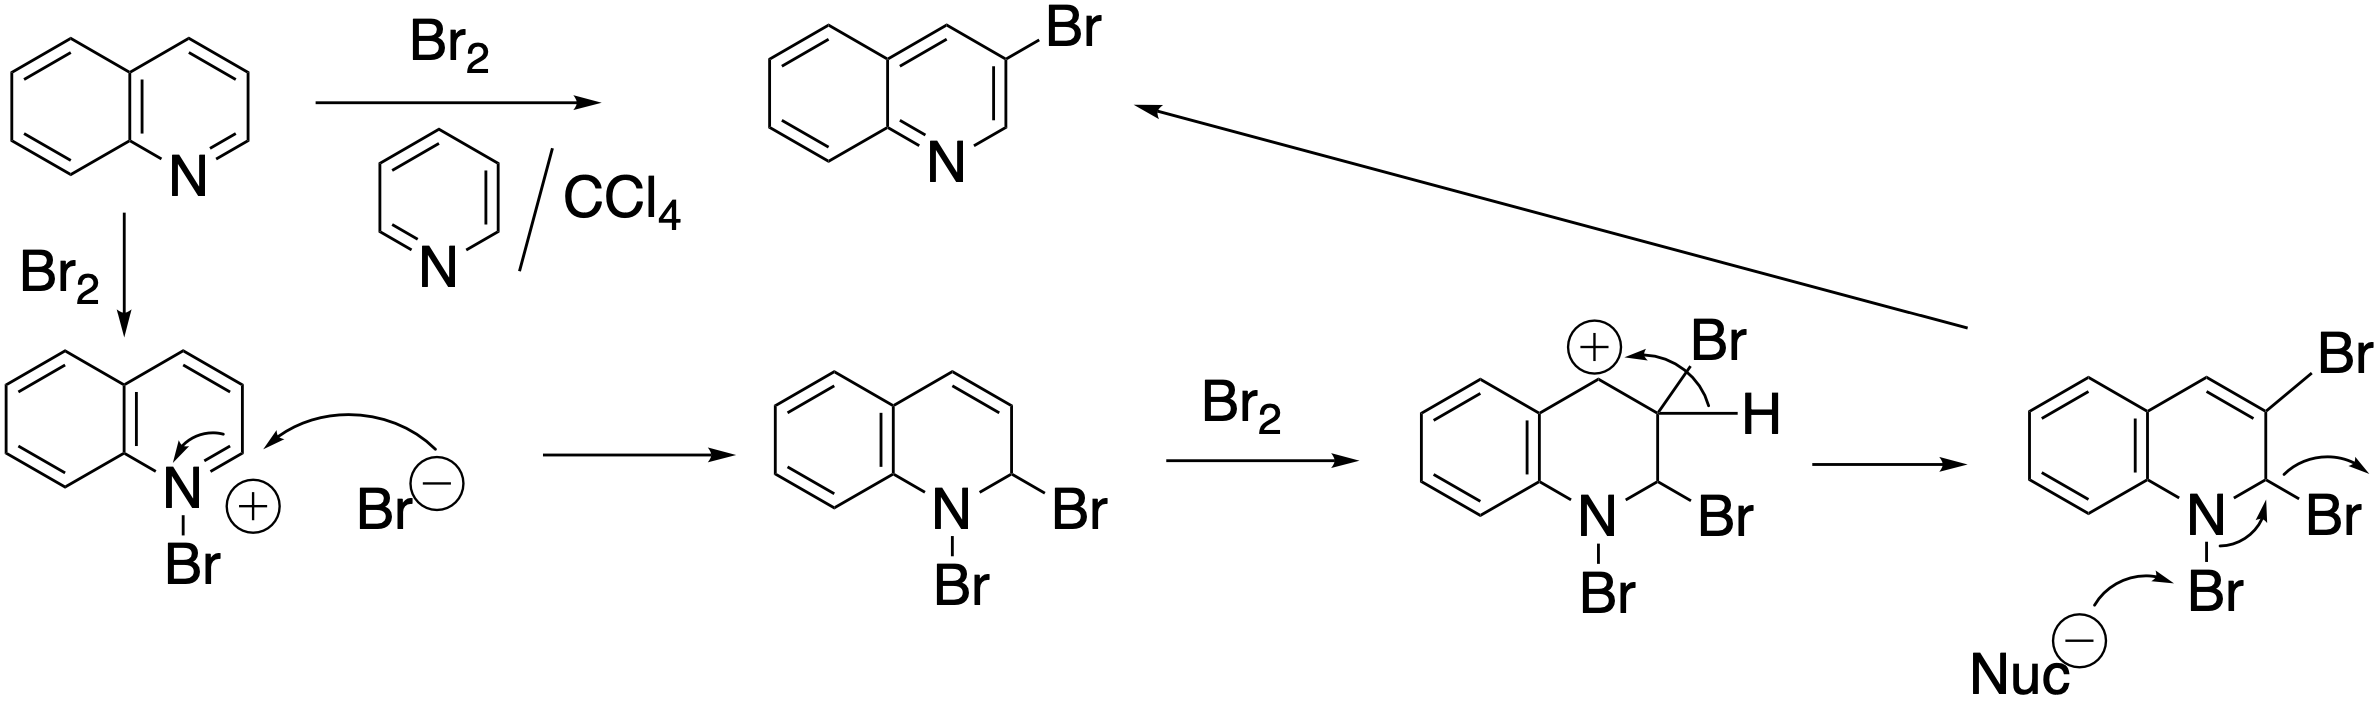
\includegraphics[width=0.8\linewidth]{QI3bromoMech.png}\\[-0.5em]
        \caption{Quinoline 3-bromination mechanism.}
        \label{fig:QI3bromoMech}
    \end{figure}
    \begin{itemize}
        \item However, the reaction mechanism is \emph{not} EAS.
        \item Indeed, this reaction is feasible only because a different mechanism is operational.
    \end{itemize}
    \item Lithiates --- followed by oxidation --- add to quinoline at the 2-position.
    \begin{figure}[h!]
        \centering
        \begin{subfigure}[b]{\linewidth}
            \centering
            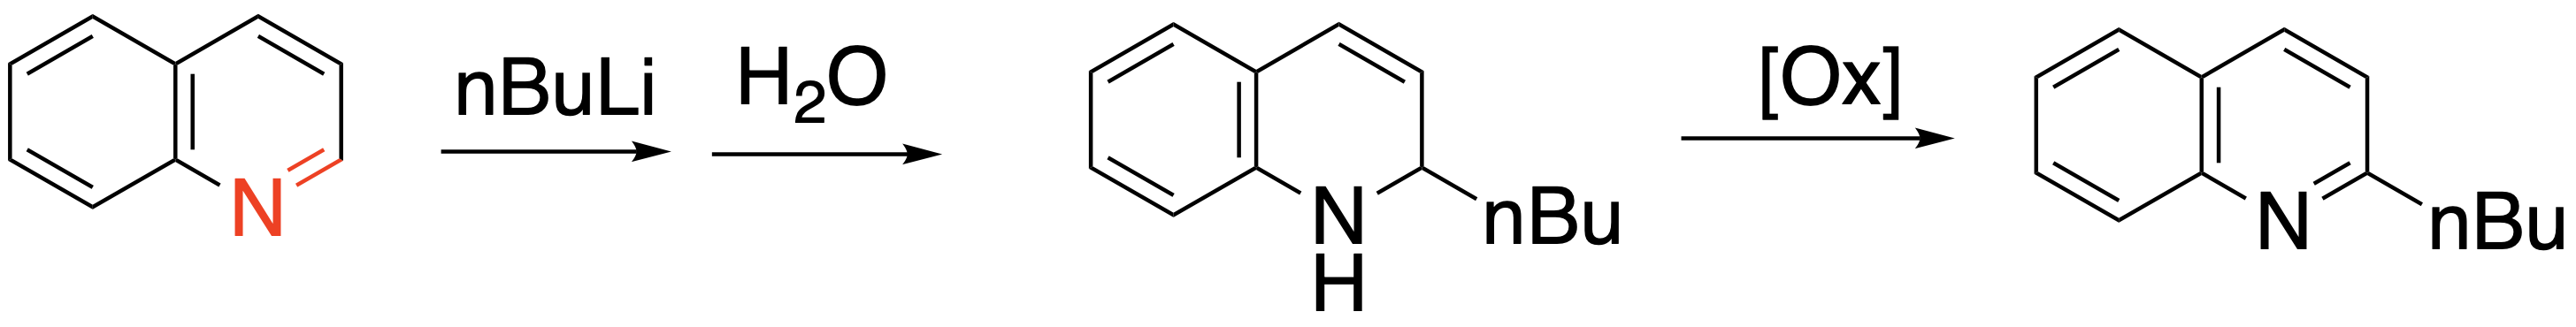
\includegraphics[width=0.63\linewidth]{QILia.png}
            \caption{Monoaddition.}
            \label{fig:QILia}
        \end{subfigure}\\[2em]
        \begin{subfigure}[b]{\linewidth}
            \centering
            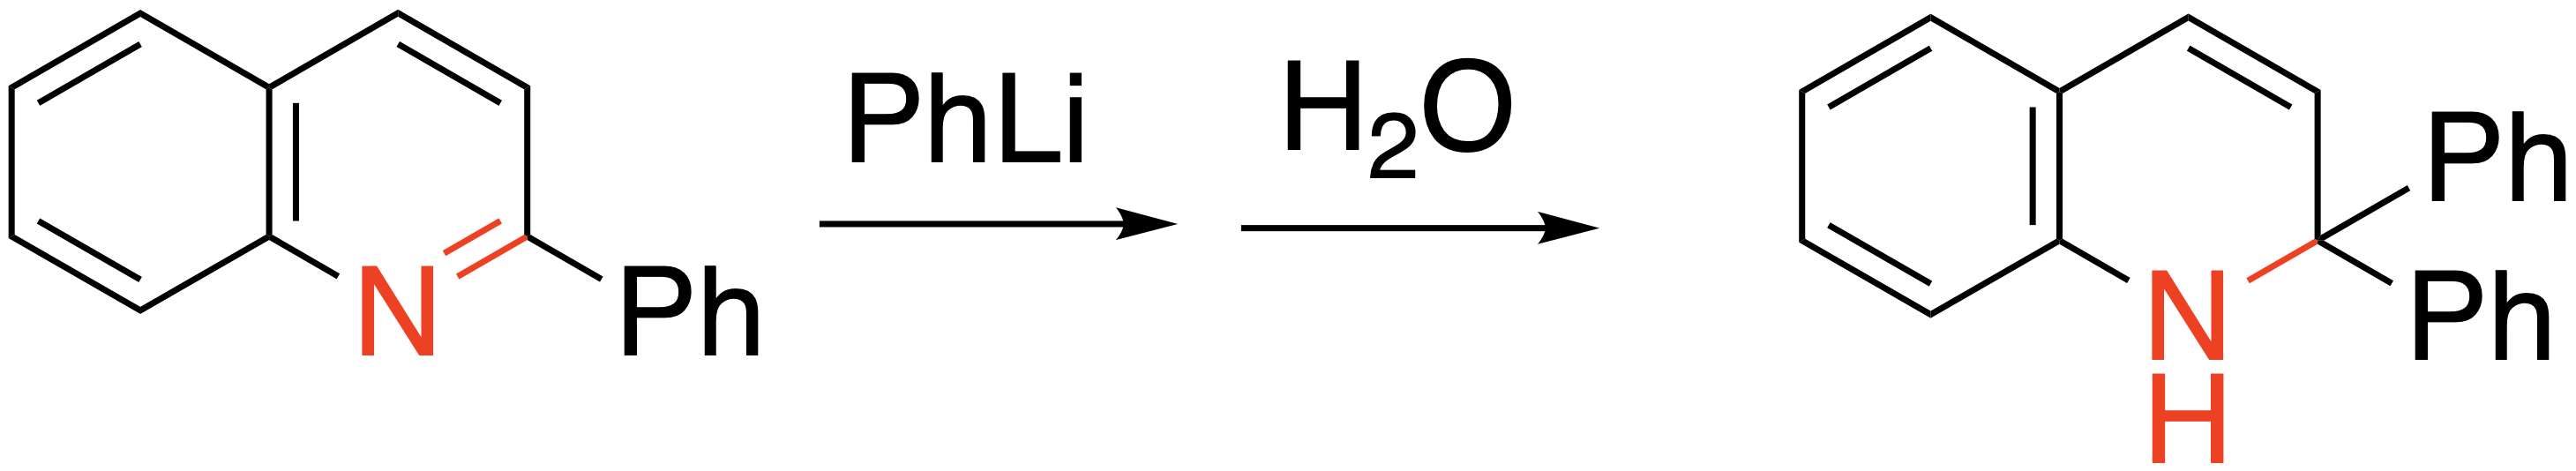
\includegraphics[width=0.41\linewidth]{QILib.png}
            \caption{Diaddition.}
            \label{fig:QILib}
        \end{subfigure}
        \caption{Lithiates add to quinoline.}
        \label{fig:QILi}
    \end{figure}
    \begin{itemize}
        \item We can also use analogous approaches to dearomatize the pyridine moiety by making a quaternary carbon.
        \item Lithium-nitrogen coordination is critical to 2-addition; otherwise, we get 4-addition.
    \end{itemize}
    \item Quinoline syntheses.
    \begin{itemize}
        \item Many different ones, many from Germany.
        \item Most common: \textbf{Skraup}, \textbf{Conrad-Limpach-Knorr}, and \textbf{Meth-Cohn} syntheses.
        \item For most of these, you start with the aniline.
        \item Common issues: Mixture of regioisomers.
    \end{itemize}
    \item Meth-Cohn quinoline synthesis.
    \begin{itemize}
        \item Proceeds via a mechanism analogous to the \textbf{Vilsmeier-Haack reaction}.
        \item Driving force: \ce{P=O} bond formation.
        \item Amide $\to$ chloroimine, tautomerizes to enamine. Then an additional carbon comes from DMF.
    \end{itemize}
    \item Quinoline hydrogenations.
    \begin{itemize}
        \item You can get some interesting chemoselectivity, enabling you to reach basically whatever you want!
        \item Reducing the benzene ring.
        \begin{itemize}
            \item Completely counterintuitive result: In the presence of an acid, you reduce the non-heterocyclic part of the quinoline heterocycle.
        \end{itemize}
        \item Reducing the heterocyclic ring, or everything: Use Raney nickel (RaNi).
        \begin{itemize}
            \item RaNi is a pyrophoric, extremely active form of nickel used for very difficult hydrogenations and desulfurizations.
            \item Under \SI{1}{\atmosphere} of \ce{H2}, you'll only hydrogenate the heterocyclic ring.
            \item Under \SI{70}{\atmosphere} of \ce{H2}, you'll hydrogenate everything (typically to the \emph{cis}-decalin derivative, but you can get some isomers).
        \end{itemize}
    \end{itemize}
    \item Most famous quinoline synthesis: The Skraup quinoline synthesis.
    \begin{itemize}
        \item Michael addition, Friedel-Crafts type cyclization, and oxidation.
        \item A series of conditions for this reaction have been optimized over time.
        \item Classic Skraup.
        \begin{itemize}
            \item Reagents: Glycerol, sulfuric acid, and \ce{As2O5} (oxidizing agent).
            \item Under acidic conditions, glycerol will lose 2 equivalents of \ce{H2O} to generate acrolein \emph{in situ}.
            \begin{itemize}
                \item Following protonation, the first step involves a hydride shift to $\beta$-hydroxyaldehyde.
                \item Then we get E\textsubscript{1} via the electron conduit to acrolein.
            \end{itemize}
            \item Why don't we just add acrolein directly?
            \begin{itemize}
                \item Glycerol is really safe and cheap, but acrolein will "polymerize if you look at it sideways."
                \item Substituted acrolein derivatives (e.g., other Michael acceptors) can be added directly with sulfuric or tosylic acid, but acrolein, itself, needs these conditions.
            \end{itemize}
            \item Using Skraup methodology, we can synthesize 1,10-phenanthroline from 8-aminoquinoline.
            \item But not super scalable: Reaction "often resulted in uncontrolled violence."
        \end{itemize}
        \item Scalable Skraup.
        \begin{itemize}
            \item Alternative: Use glycerol in the presence of iron sulfate, a strong acid (e.g., methane sulfonic acid), and a strong oxidant (deprotonated sulfonic acid).
            \begin{itemize}
                \item The use of this particular oxidant makes separation easier at the end.
                \item This is an unusual use of a nitro group as an oxidizing agent; not often used, but was recently by Baran.
            \end{itemize}
            \item Once acrolein is generated \emph{in situ}, it undergoes Michael addition. Then we get Friedel-Crafts reactivity, followed by oxidation.
            \item This method was used to synthesize a PDE4 inhibitor.
        \end{itemize}
    \end{itemize}
    \item Misc. quinoline derivative syntheses.
    \begin{itemize}
        \item \textbf{Combes} (quinoline synthesis): Aniline condenses with a $\beta$-diketone, followed by intramolecular acid-promoted Friedel-Crafts cyclization.
        \item \textbf{Conrad-Limpach-Knorr} (quinolone synthesis): The mechanism involves a Combes-analogous condensation with a $\beta$-ketoester, followed by Friedel-Crafts cyclization.
        \begin{itemize}
            \item Sulfuric acid gives the 2-quinolone product.
            \item Heat gives the 4-quinolone product.
            \item We'll discuss this difference later!
        \end{itemize}
        \item Used to make compounds that fight botulism, malaria, and ebola.
        \begin{itemize}
            \item One important reagent used in some syntheses is \textbf{Eaton's reagent}.
        \end{itemize}
    \end{itemize}
    \item \textbf{Eaton's reagent}: \ce{MeSO3H} + \ce{P2O5}.
    \begin{itemize}
        \item This is a variation on PPA from last time. Easier to work with an quantitate.
    \end{itemize}
    \item Making a KRAS inhibitor.
    \begin{itemize}
        \item KRAS is a particularly virulent form of cancer for which inhibitors have not come on the market until recently.
        \item The starting material is a trisubstituted anline that is probably not cheap.
        \item Selectively (or selectively enough) chlorinate this SM.
        \begin{itemize}
            \item On an exam, Steve will never ask us to think that we could do this selectively.
            \item It's not obvious to him that we would chlorinate where we do, but we \emph{should} be able to draw a mechanism!! (This is basically 5.12 chem.)
        \end{itemize}
        \item \textbf{Meldrum's acid} and a trimethyl orthoester condense into a new reagent.
        \begin{itemize}
            \item This reagent is very prone to nucleophilic attack, so we get a Michael-type addition-elimination condensation with the aniline.
        \end{itemize}
        \item Then heating the mixture to boiling using Dowtherm as a solvent causes the substrate to collapse to the quinolone.
        \begin{itemize}
            \item The mechanism for this is at the bottom in the box.
            \item Note that at high temperatures, Meldrum's acid is known to undergo a pericyclic decomposition to a ketene, \ce{CO2}, and acetone; evidently, only acetone gets kicked out here, not \ce{CO2}.\footnote{\href{https://en.wikipedia.org/wiki/Meldrum's_acid\#Synthesis_of_ketenes}{Wikipedia}. Note also that Meldrum's acid is so strong because the conformational restriction caused by the ring forces the $\alpha$-proton to undergo $\sigma_{\ce{CH}}\to\pi^*_{\ce{CO}}$ donation.}
            \item In fact, it appears that the whole mechanism in the box plausibly occurs via a sequence of pericyclic reactions.
        \end{itemize}
        \item Nitric acid then gives nitration.
        \item \ce{POCl3} chlorinates the ketone and aromatizes the system.
        \item Pretty selective S\textsubscript{N}Ar occurs, even with a hindered piperazine.
        \item A note of the mechanism of action: Acrylimides (top of the finished molecule) are thought to give Michael addition with DNA.
    \end{itemize}
    \item \textbf{Friedlander} (quinoline synthesis).
    \begin{itemize}
        \item Retrosynthetic disconnections: An alkene disconnects into a carbanion equivalent and a carbonyl, and an imine disconnects into an amine and a carbonyl.
        \begin{itemize}
            \item Very rational.
        \end{itemize}
        \item Subject to regiocontrol issues.
        \begin{itemize}
            \item McWilliams (at Pfizer) did a very careful study, and was able to use an organocatalyst to get 90\% selectivity for one regioisomer.
        \end{itemize}
        \item Aside: Scalability.
        \begin{itemize}
            \item 90\% selectivity may not sound great to us.
            \item But as long as we can reject the unwanted isomer via recrystallization or derivitization (not chromatography), this is much better than a 4-step synthesis that requires complicated/expensive reagents or conditions.
        \end{itemize}
        \item This chemistry is generalizable, as well; see the reaction at the bottom of the slide.
        \item Anytime the symbol "OEi" appears in a slide, that means "$\Delta$."
    \end{itemize}
    \item Example synthesis: A MS drug by UCB (a Belgian pharmaceutical company).
    \begin{itemize}
        \item Starting material: A nitro-phenylalanine derivative.
        \item Condensation to the amide with a variant of Yamaguchi's reagent.
        \item Reduction of the nitro group to the corresponding aniline.
        \item Condensation with a dichlorobenzaldehyde to form the imine.
        \item \textbf{Pavarov reaction} with a good leaving group.
        \begin{itemize}
            \item Specifically, 2-pyrrolidone leave under oxidative conditions.
        \end{itemize}
        \item Lastly, we hydrolyze the ester to an acid.
        \item Two solvent swaps.
        \begin{itemize}
            \item These are supposed to purge impurities using washes; we rarely do this in academia.
            \item Switching to ACN gets rid of water, and switching to heptane gets rid of the ACN because nonpolar molecules don't stick to polar molecules and can thus be removed well under vacuum.
        \end{itemize}
    \end{itemize}
    \item This concludes our discussion of quinolines for the time being.
    \item We now discuss isoquinolines.
    \item Isoquinolines.
    \begin{itemize}
        \item It's easier to do chemistry on their nonheterocyclic part.
        \begin{itemize}
            \item For example, nitration and bromination most frequently occur at the 5- and 8-positions.
        \end{itemize}
        \item Unsurprisingly, the Chichibabin and lithiate/oxidation reactions work again.
        \begin{itemize}
            \item Nucleophiles will \emph{always} add at the position between the nitrogen and other aromatic ring.
            \item With the dichloro species, you should be very confident you can do the addition to this position.
            \item This may show up on an exam!!
        \end{itemize}
    \end{itemize}
    \item Isoquinoline syntheses.
    \begin{itemize}
        \item \textbf{Pomeranz-Fritsch} (isoquinoline synthesis): A condensation/Friedel-Crafts between an aldehyde and the synthetic equivalent of 2-aminoacetaldehyde.
        \begin{itemize}
            \item Like acrolein, we can't use 2-aminoacetaldehyde raw because it self-condenses.
            \item Treatment with acid forms the heteroatom-stabilized carbocation that then does Friedel-Crafts chemistry.
        \end{itemize}
        \item We can also do \ce{C-N} cross-coupling (which we'll discuss later).
        \item \textbf{Bischler-Napieralski} (isoquinoline synthesis).
        \begin{itemize}
            \item Make an amide.
            \item Then use \ce{POCl3} to access the nitrilium ion via a chloroimine-type mechanism.
            \item The chloroimine is in no-bond resonance with the nitrilium ion, which is very active in Friedel-Crafts type chemistry.
        \end{itemize}
        \item \textbf{Pictet-Gams} variation of the Bischler-Napieralski reaction.
        \begin{itemize}
            \item Start with a benylic alcohol.
            \item Thus, you've pre-installed your oxidation! That's the advantage.
            \item The disadvantage is getting the substrate.
        \end{itemize}
    \end{itemize}
    \item \textbf{Pictet-Spengler} reaction.
    \begin{itemize}
        \item From early 20th century Germany.
        \item Phenethyl amine and an aldehyde condense and cyclize.
        \item Generalizable to other substrates.
        \item Proposed mechanism: The iminium ion produced during condensation cyclizes.
        \begin{itemize}
            \item This can occur via Friedel-Crafts type chemistry, or via a more complicated mechanism with shifts depending on the substrate.
            \item In the example shown, it does make more sense that the more nucleophilic position would initially attack the iminium ion, before rearrangement!
        \end{itemize}
    \end{itemize}
    \item Example synthesis: Idorisia needed to make a pretty simple compound, but making it at scale was hard.
    \begin{itemize}
        \item Process groups "compete" multiple routes for cost-efficiency, safety, and reliable access to reagents from multiple sources.
        \begin{itemize}
            \item Because the bigshots will say, "we need 5 kilos in 3 months. If that goes well, 50 kilos 6 months after that. If that goes well, a tonne a year after that."
            \item Then the process chemists will start with what they know works, and then they'll refine at cost, scale (e.g., issues with exotherms), issues with buying materials or catalysts, etc.
        \end{itemize}
        \item Route-scouting summary.
        \begin{itemize}
            \item None of the routes use particularly fancy chemistry. Route A uses really old chemisty (\textbf{Balz-Schiemann} reaction).
        \end{itemize}
        \item Route A overview.
        \begin{itemize}
            \item \ce{POCl3} probably gave a side product that was hard to reject, so they use \ce{POCl(OPh)2}.
            \item Lots of energy put into optimizing this route, so Steve guesses it must have been a really desirable starting material.
            \item Primary amide to Hofmann rearrangement.
            \item Diazitized, then classic Balz-Schiemann.
        \end{itemize}
        \item Route B.
        \begin{itemize}
            \item On small scale, we can do a Stille reaction.
            \begin{itemize}
                \item We could also do tin/lithium exchange and something else (??) to get to a more scalable intermediate.
                \item Then we can get to a desired $\alpha$-fluoro reagent.
            \end{itemize}
            \item However, there's a better bucket chemistry approach.
            \begin{itemize}
                \item Carboxylic acid to acyl malonate. Very acidic, hence easily able to fluorinate.
                \item Then double hydrolysis/decarboxylation to form the $\alpha$-fluoro intermediate.
            \end{itemize}
            \item We then use an amide acetal, a species analogous to an orthoester that is derived from DMF. This forms a \textbf{vinylogous}\footnote{\href{https://en.wikipedia.org/wiki/Vinylogy}{Wikipedia}.} amide, an enamine-type compound.
            \item Then under hydrogenation conditions, a quinoline \emph{N}-oxide is formed. This then gets hydrogenated down to form another intermediate.
            \item At this point, we excise the alcohol \ce{OH} with \ce{POCl3} and reduction.
            \begin{itemize}
                \item This is a \textbf{transfer hydrogenation}, with formate is a hydrogen source
            \end{itemize}
            \item Aside: Pharma companies have tight controls on hydrogen; you can't even use a balloon unless you go to a special room. Avoid until scale-up!
        \end{itemize}
        \item In the end, they chose to use Route C.
        \begin{itemize}
            \item It's better to not use (very expensive) Selectfluor.
        \end{itemize}
    \end{itemize}
    \item We now move onto diazenes.
    \begin{itemize}
        \item Key diazenes.
        \begin{itemize}
            \item Benzene derivatives: Pyridazine, pyrimidine, pyrazine.
            \item Quinoline derivatives: Cinnoline, phthalazine, quinazoline, quinoxaline.
            \item The benzene derivatives aren't too common, but the benzanulated heterocycles are very common in pharmaceuticals.
        \end{itemize}
        \item Important characteristics.
        \begin{itemize}
            \item All of the effects of adding one nitrogen to benzene to make pyridine are intensified.
            \item Pyridazine, pyrimidine, and pyrazine are colorless liquids that are water soluble.
            \item Nucleophilic addition is much easier.
            \item Electrophilic addition is much harder.
            \item The compounds are much less nucleophilic and basic.
        \end{itemize}
        \item The $\alpha$-effect in pyridazine makes it easier to protonate than pyrimidine.
    \end{itemize}
    \item Halo-diazenes.
    \begin{itemize}
        \item For the purposes of this class, assume that 4-chloro will react faster than 2-chloro.
        \begin{itemize}
            \item Sharon Neufeldt (Montana State) had a nice paper in JACS recently with an exception to this \parencite{bib:Neufeldt}.
        \end{itemize}
        \item These can be very fast S\textsubscript{N}Ar reactions.
        \item Handwavey reason: Double $\alpha$-effect is worse than one lone pair Coulombic problem.
    \end{itemize}
    % \item We'll now do some practice problems.
    \item Problem 1.
    \begin{figure}[H]
        \centering
        \footnotesize
        \begin{subfigure}[b]{\linewidth}
            \centering
            \schemestart
                \chemfig{*6(-N=(-(=[6]O)-[:30]OH)-=(-[,,,,opacity=0]\phantom{Cl})-=)}
                \arrow{->[\ce{SOCl2} (xs)][$\Delta$]}[,1.5]
                \chemfig{*6(-N(-[6,0.7,,,opacity=0]{\bullet HCl})=(-(=[6]O)-[:30]Cl)-=(-Cl)-=)}
            \schemestop
            \caption{The reaction.}
            \label{fig:TTQPy4Cla}
        \end{subfigure}\\[1.8em]
        \begin{subfigure}[b]{\linewidth}
            \centering
            \schemestart
                \chemfig{*6(-N=(-(=[6]O)-[:30]OH)-=-=)}
                \arrow{->[\ce{SOCl2}][-\ce{SO2}, \ce{Cl-}]}[,1.4]
                \chemfig{*6(-@{2N}\charge{-90=\:}{N}=(-(=[6]O)-[:30]Cl)-=-=)}
                \arrow{->[{\chemfig[atom sep=1.4em]{Cl-[:30]@{3S}S(=[@{31}2]O)-[@{32}:-30]@{3Cl}Cl}}][-\ce{Cl-}]}[,1.6]
                \chemfig{*6(-@{4N}\charge{[extra sep=4pt]-150=$\oplus$}{N}(-[6]S(=[:-150]O)-[:-30]Cl)=[@{43}](-(=[6]O)-[:30]Cl)-[@{42}]=[@{41}]@{4C}-=)}
                \arrow{->[*{0}\chemfig{@{5Cl}\charge{[extra sep=4pt]45=$\ominus$}{Cl}}]}[-90,0.8]
                \chemfig{*6(-N(-[@{65}]@{6S}S(=[:-150]O)-[:-30]Cl)-[@{64,0.4}](-(=[6]O)-[:30]Cl)=[@{63}]-[@{62}](-[:70]Cl)(-[@{61}:110]@{6H}H)-=)}
                \arrow{->[\chemfig{@{7Cl}\charge{[extra sep=4pt]45=$\ominus$}{Cl}}][-\ce{SOCl-}]}[180,1.2]
                \chemfig{*6(-N(-[6,0.7,,,opacity=0]{\bullet HCl})=(-(=[6]O)-[:30]Cl)-=(-Cl)-=)}
            \schemestop
            \chemmove{
                \draw [curved arrow={5pt}{2pt}] (2N)
                    to[out=-90,in=180] ++(1,-0.9)
                    to[out=0,in=150] (3S)
                ;
                \draw [curved arrow={4pt}{4pt}] ([xshift=1pt,yshift=-4pt]31) to[out=60,in=120,looseness=40] ([xshift=-1pt,yshift=-4pt]31);
                \draw [curved arrow={2pt}{2pt}] (32) to[bend left=80,looseness=3] (3Cl);
                % 
                \draw [curved arrow={11pt}{2pt}] (5Cl) to[out=45,in=90,out looseness=3.3] (4C);
                \draw [curved arrow={4pt}{2pt}] (41) to[bend right=60,looseness=1.5] (42);
                \draw [curved arrow={4pt}{2pt}] (43) to[bend right=60,looseness=2] (4N);
                % 
                \draw [curved arrow={11pt}{2pt}] (7Cl) to[out=45,in=180] (6H);
                \draw [curved arrow={2pt}{2pt}] (61) to[out=-150,in=-140,looseness=2] (62);
                \draw [curved arrow={4pt}{2pt}] (63) to[bend right=60,looseness=1.7] (64);
                \draw [curved arrow={2pt}{2pt}] (65) to[bend right=70,looseness=2.5] (6S);
            }
            \caption{The mechanism.}
            \label{fig:TTQPy4Clb}
        \end{subfigure}
        \caption{TTQ: Pyridine 4-chlorination.}
        \label{fig:TTQPy4Cl}
    \end{figure}
    \begin{itemize}
        \item Convert to the acid chloride.
        \item Activate the pyridine by reacting it with the best electrophile in solution; experimental studies show that it's not protonation here! Plus, protonation would make hydride your leaving group, which is much worse than \ce{SOCl-}.
        \item Chloride may not be the base that does the final deprotonation, but we want the hydrochloride in the end so it's good to show that. If not chloride, subsequent proton exchange gives hydrochloride.
        \item Fate of sulfur compound is unknown, so \ce{SOCl-} is some kind of leaving group. That was our hint to use a sulfur electrophile to activate the ring.
    \end{itemize}
    \item Problem 2.
    \begin{figure}[H]
        \centering
        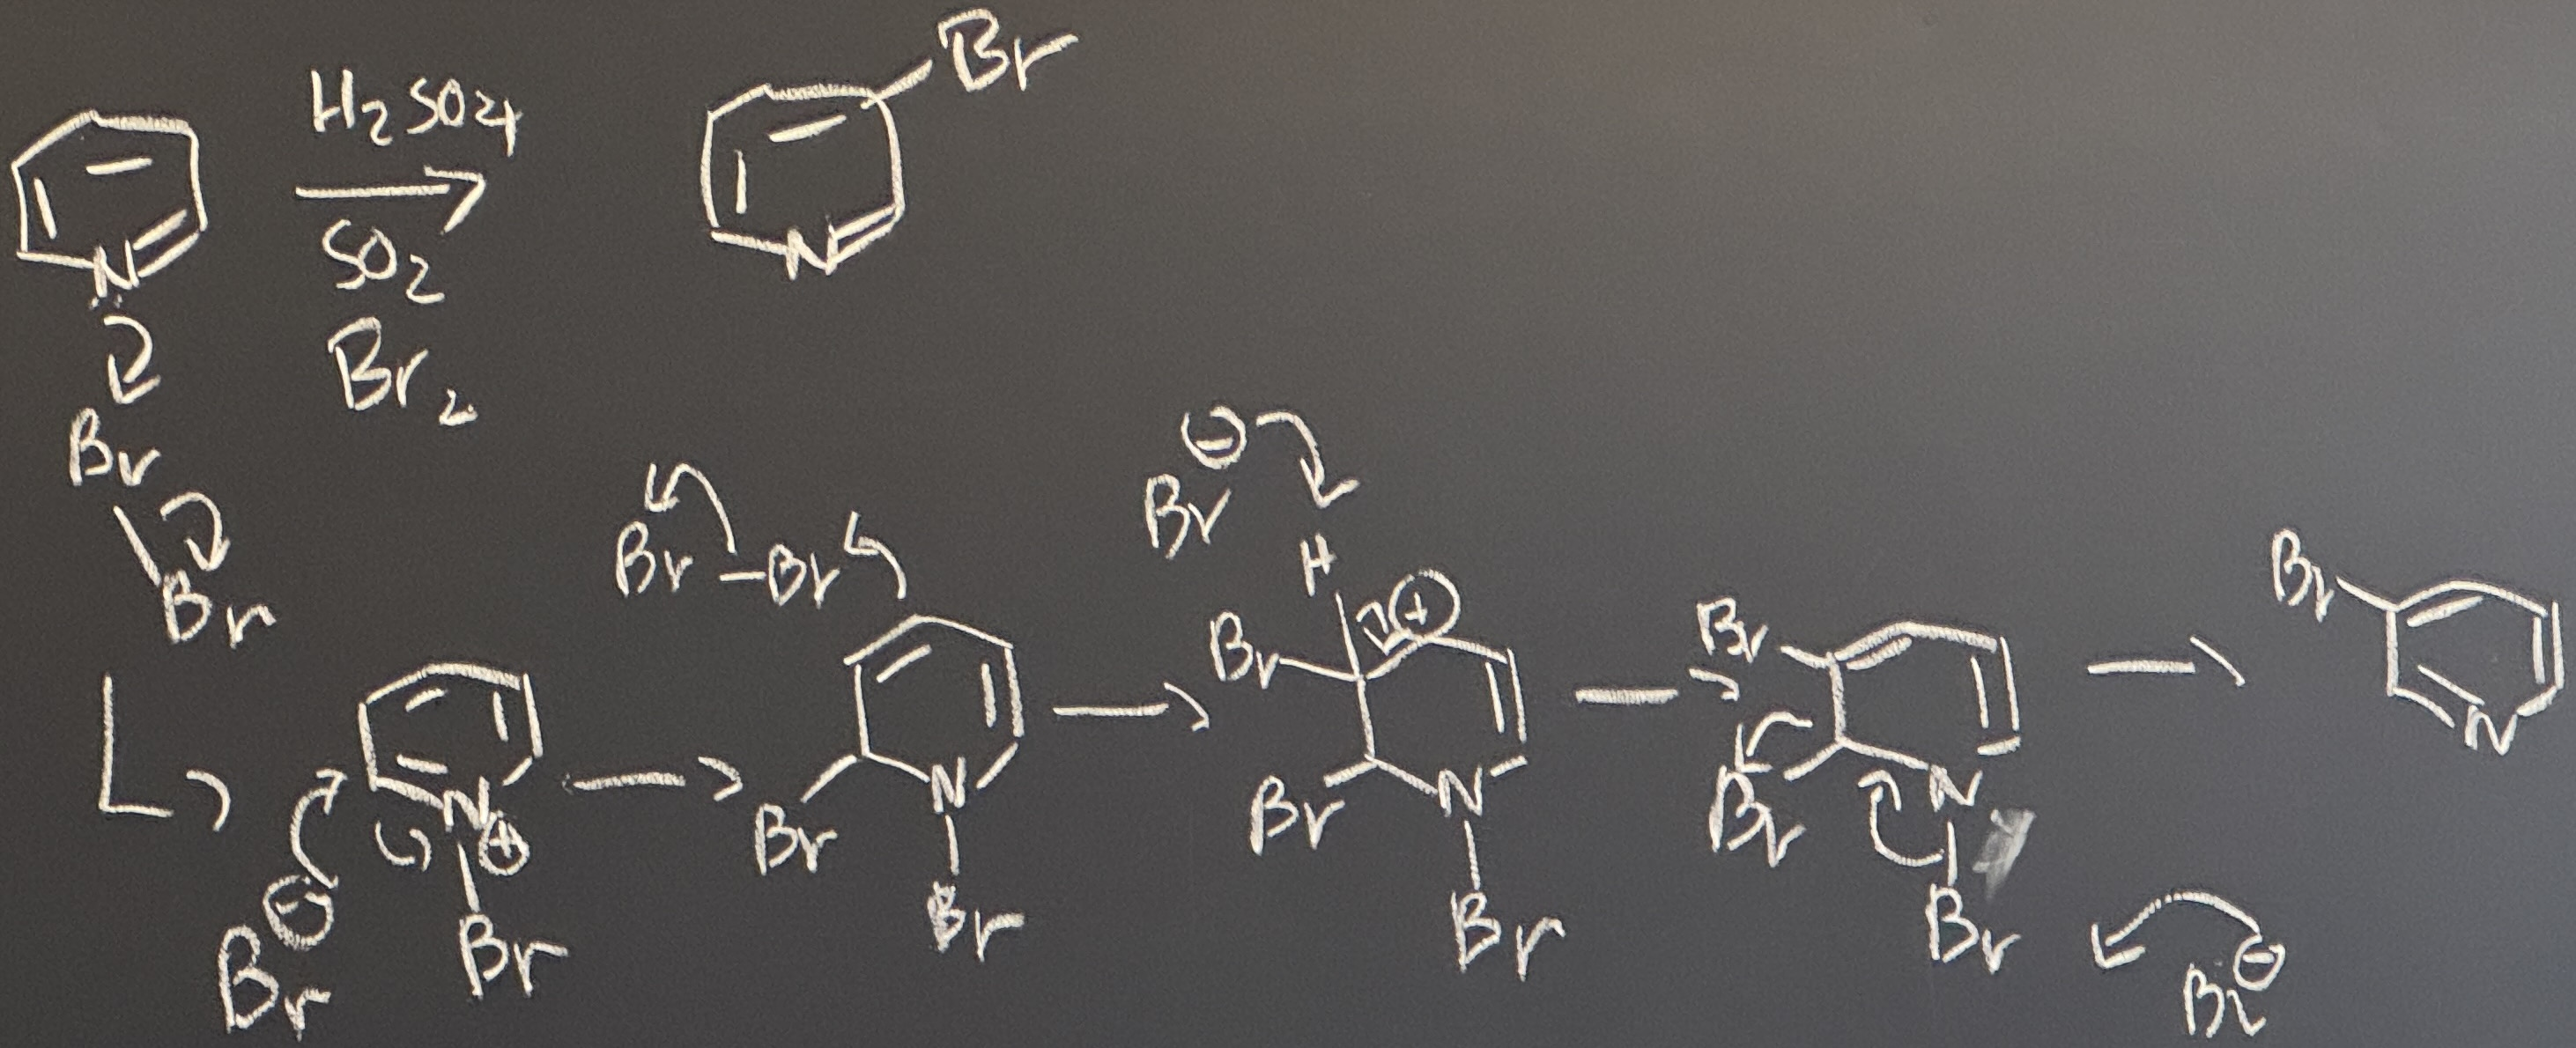
\includegraphics[width=0.6\linewidth]{TTQPy3Br.JPG}
        \caption{TTQ: Pyridine \emph{meta}-bromination.}
        \label{fig:TTQPy3Br}
    \end{figure}
    \begin{itemize}
        \item Uses bromination mechanism from class (see Figure \ref{fig:QI3bromoMech}).
        \item Oleum could be \ce{SO2} or \ce{SO3}.
        \item \ce{Br-} can remove either bromine in the last step.
        \item This gets full credit; it is great, but for the second bromination, it may make more sense to put the bromine on the other side of the compound; the 1,2-dibromide is unfavorable.
        \begin{itemize}
            \item Principle: Large halides on contiguous carbons is just very challenging.
        \end{itemize}
        \item Unclear what the \ce{SO2} does.
        \item Electrophilic reaction $\to$ nucleophilic reaction with dearomatization.
    \end{itemize}
\end{itemize}



\section{Pyrimidines and Pyrroles}
\begin{itemize}
    \item \marginnote{2/13:}Syntheses of pyrimidines.
    \begin{itemize}
        \item Several disconnections once again.
        \item Most important ones: The $[3+3]$ disconnections, especially the \textbf{Pinner reaction}.
        \item Pinner reaction.
        \begin{itemize}
            \item You make an \textbf{amidine}, typically by adding a sodamide (\ce{NH2-}) to a nitrile.
        \end{itemize}
        \item \textbf{Grimaux} (pyrimidine synthesis).
        \begin{itemize}
            \item Makes barbituric acid (part of barbituates).
            \item Equivalent of a diacid chloride plus a urea.
            \item Then can be converted into halides using reactions we've discussed such as \ce{POCl3}.
        \end{itemize}
        \item \textbf{Biginelli} (pyrimidine synthesis).
        \begin{itemize}
            \item Ignored for 125 years.
            \item Became popular when people wanted libraries of heterocycles.
            \item Popular because you can mix and match $\beta$-ketoesters, aldehydes, and ureas.
            \item Mechanistically, you begin with a \textbf{Knoevenagel condensation} (aldol variant). This gives a species very activated torward Michael addition, so urea can add twice.
            \item "Urea has the solubility of brick dust," so you need a quite active solvent mixture to get at least some of it in solution.
        \end{itemize}
        \item \textbf{Ziegenbein-Franke} (pyrimidine synthesis).
        \begin{itemize}
            \item Very young; about 60 years old.
            \item Think about the mechanism of ketone to $\beta$-chloroaldehyde (once again, a 1,3-biselectrophile)!!
            \item The $\beta$-chloroaldehyde is then pyrolized with formamide.
            \item Mechanism: Michael addition, transitive imine formation, addition-elimination to lose \ce{H2O}.
        \end{itemize}
        \item \textbf{Pinner} (reaction).
        \begin{itemize}
            \item Acidic reaction with a nitrile gives a \textbf{Pinner salt}.
            \item Either hydrolyse or convert to the amidine.
            \item Several 1,3-bisnucleophiles can be treated with 1,3-biselectrophiles (typically a $\beta$-dicarbonyl, but can be others) in this manner.
        \end{itemize}
    \end{itemize}
    \item Addendum: Vilsmeier-Haack type chloroformylation mechanism.
    \begin{figure}[H]
        \centering
        \begin{subfigure}[b]{\linewidth}
            \centering
            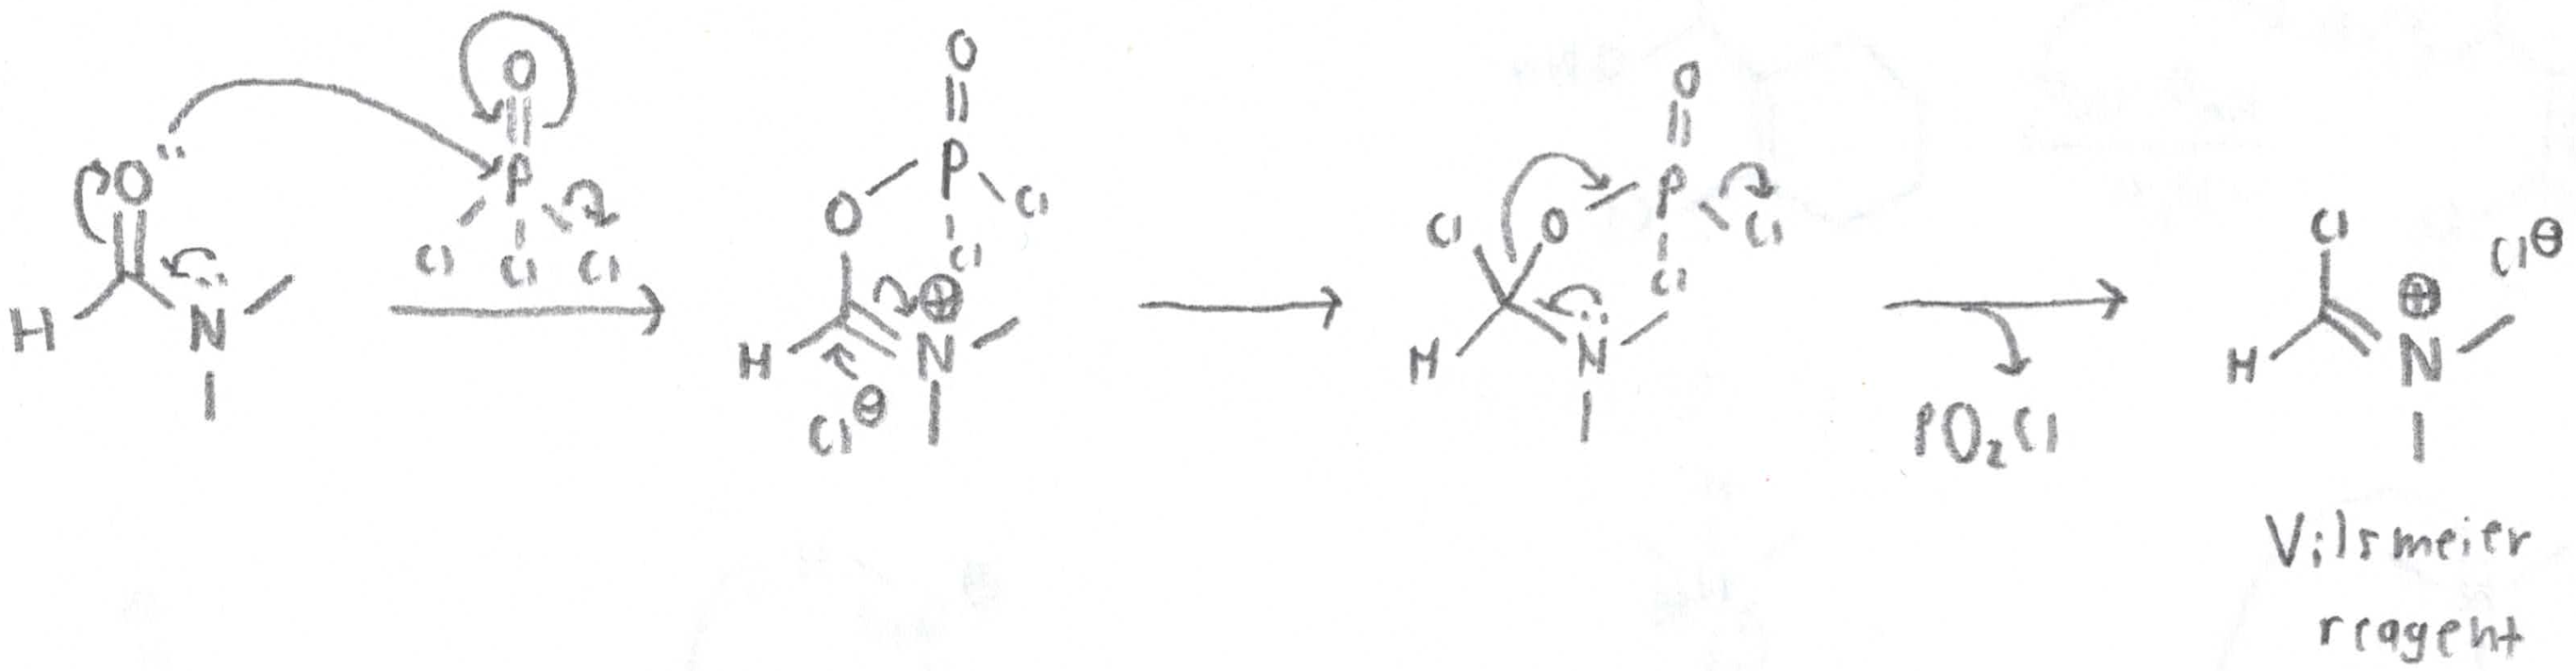
\includegraphics[width=0.75\linewidth]{VHClCHOMecha.png}
            \caption{Preparation of the Vilsmeier reagent.}
            \label{fig:VHClCHOMecha}
        \end{subfigure}
    \end{figure}
    \begin{figure}[h!]
        \ContinuedFloat
        \centering
        \begin{subfigure}[b]{\linewidth}
            \centering
            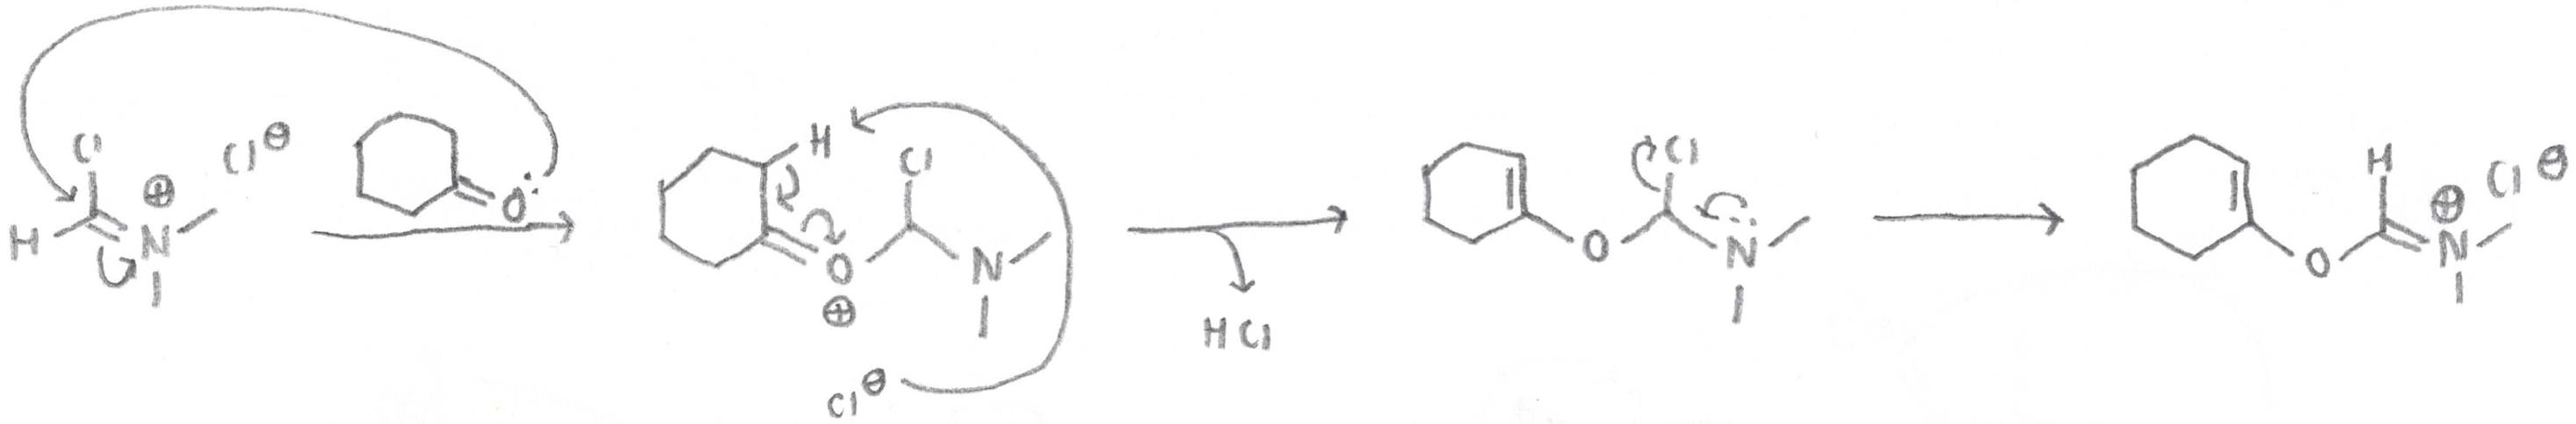
\includegraphics[width=0.9\linewidth]{VHClCHOMechb.png}
            \caption{Hydrochloric acid libration for autocatalysis of the keto-enol tautomerization.}
            \label{fig:VHClCHOMechb}
        \end{subfigure}\\[2em]
        \begin{subfigure}[b]{\linewidth}
            \centering
            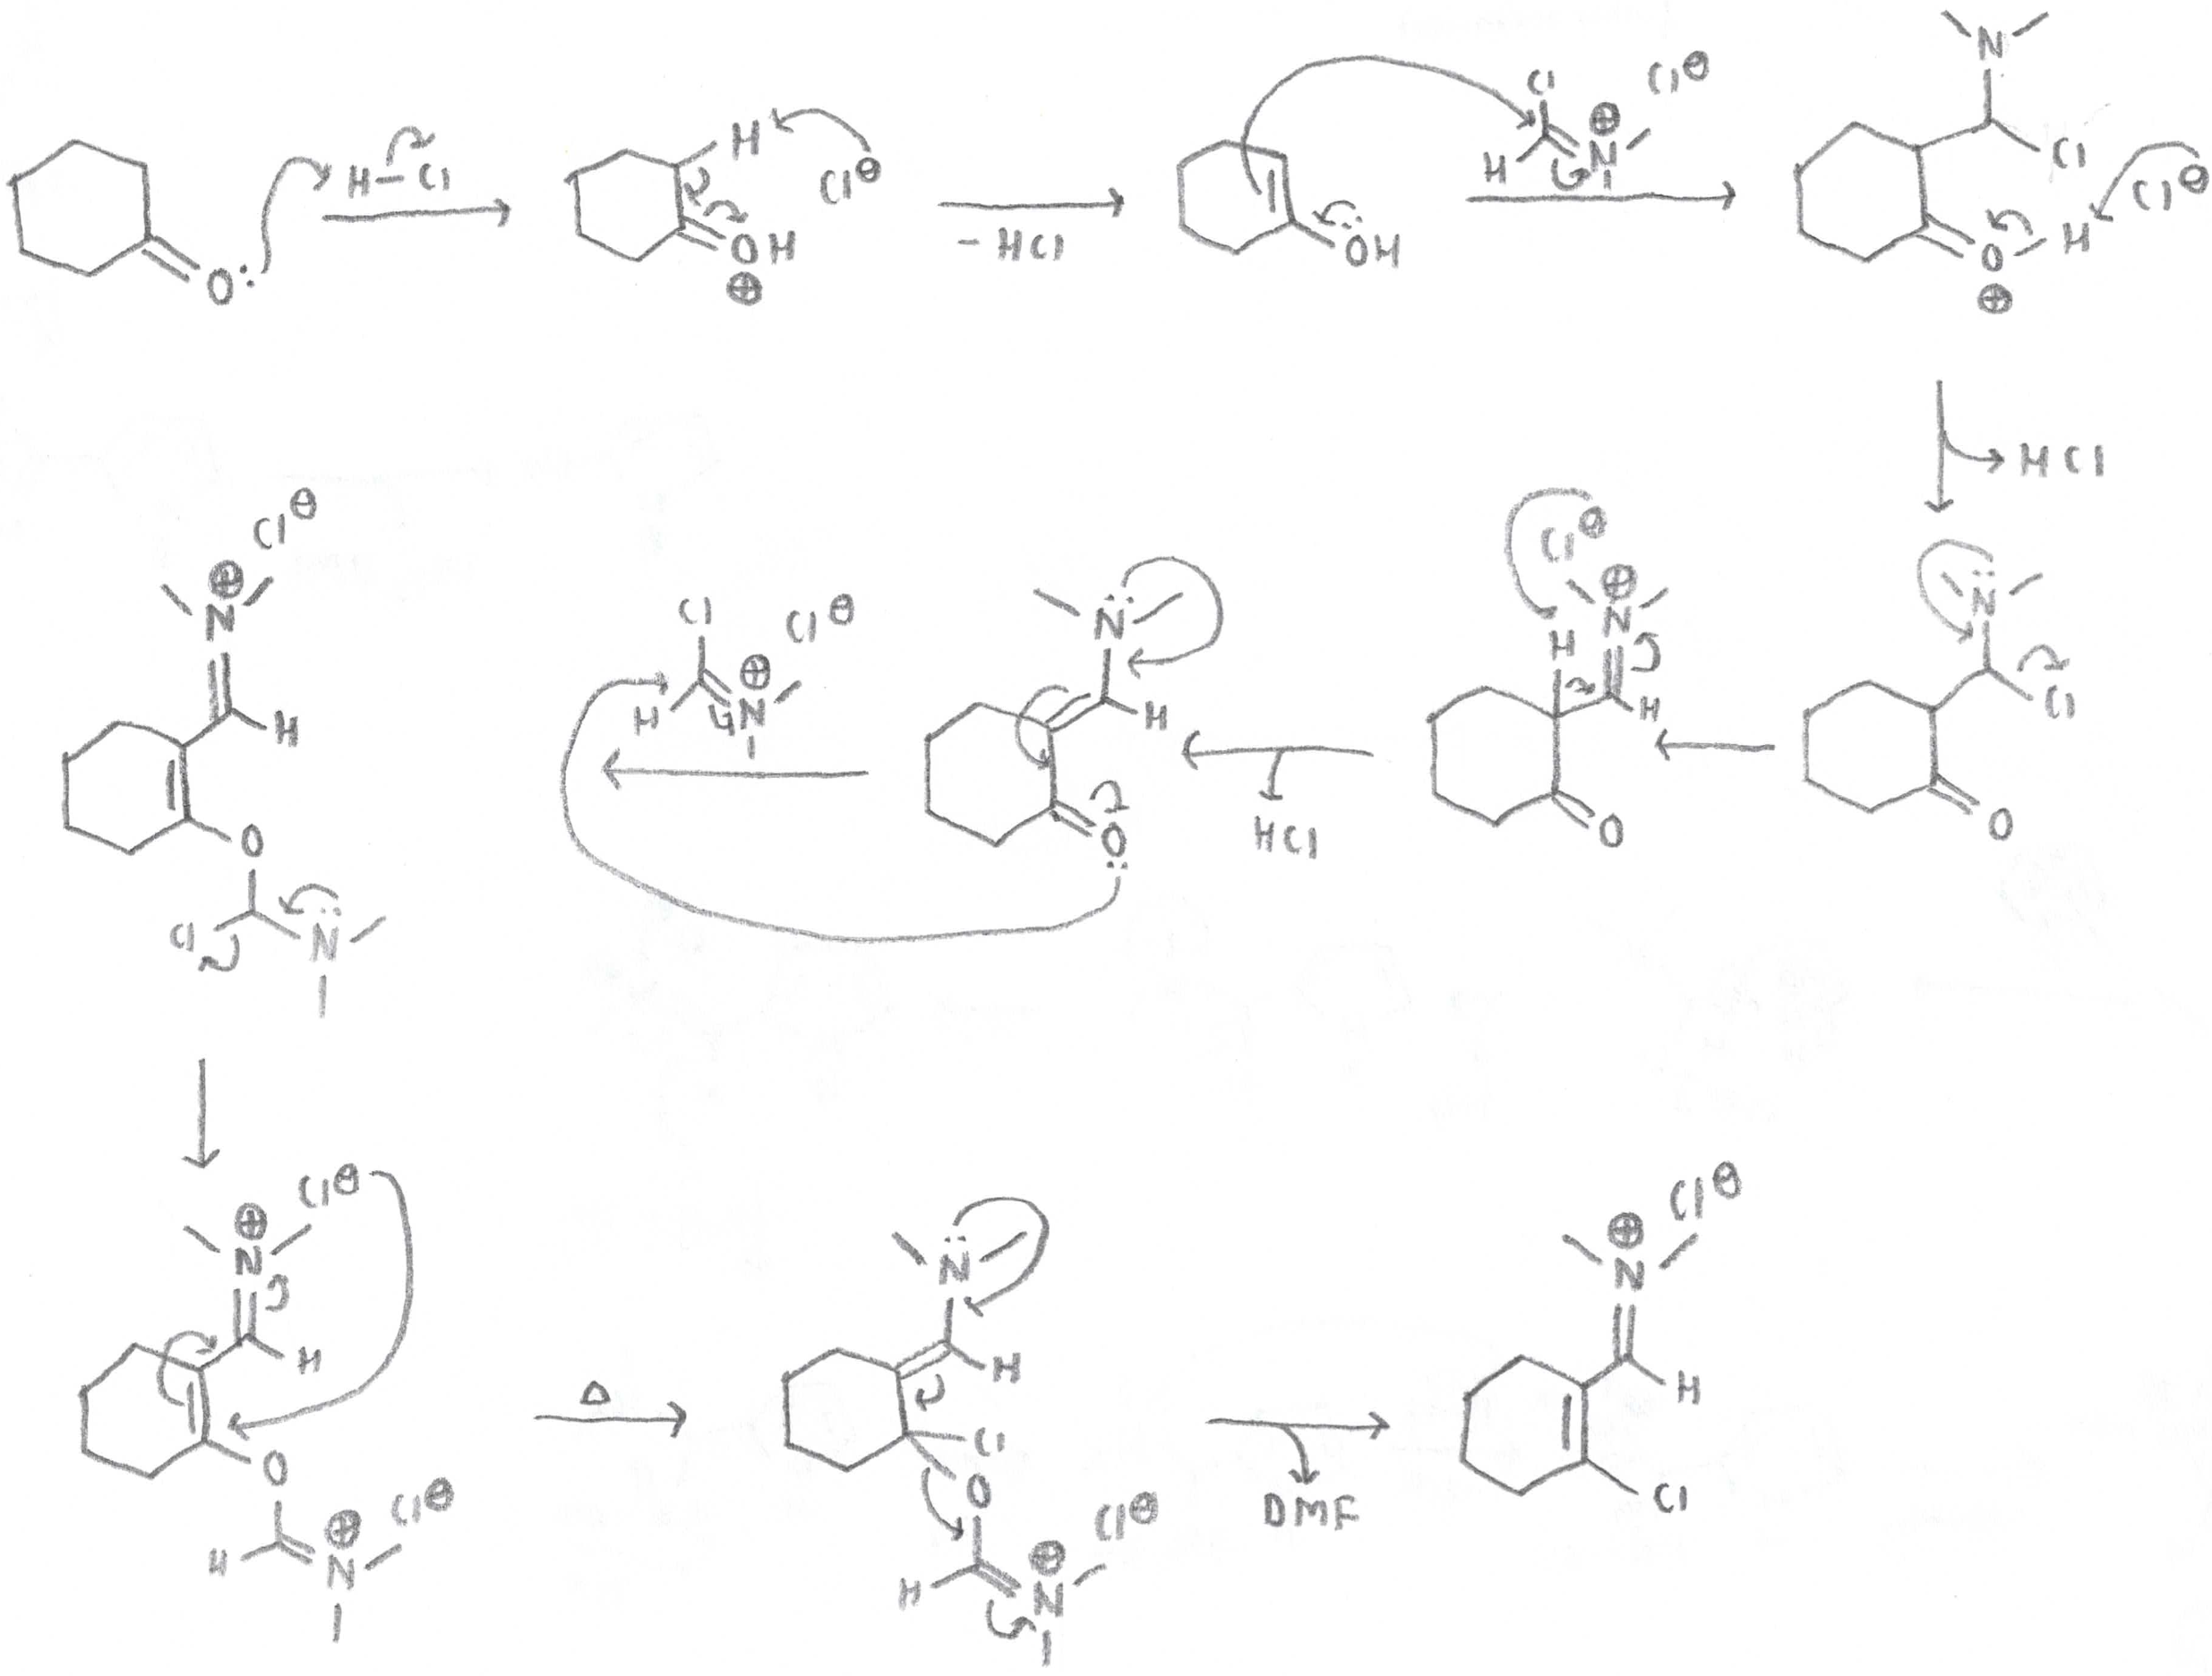
\includegraphics[width=0.8\linewidth]{VHClCHOMechc.png}
            \caption{Formation of the $\beta$-chloroacryliminium chloride salt.}
            \label{fig:VHClCHOMechc}
        \end{subfigure}\\[2em]
        \begin{subfigure}[b]{\linewidth}
            \centering
            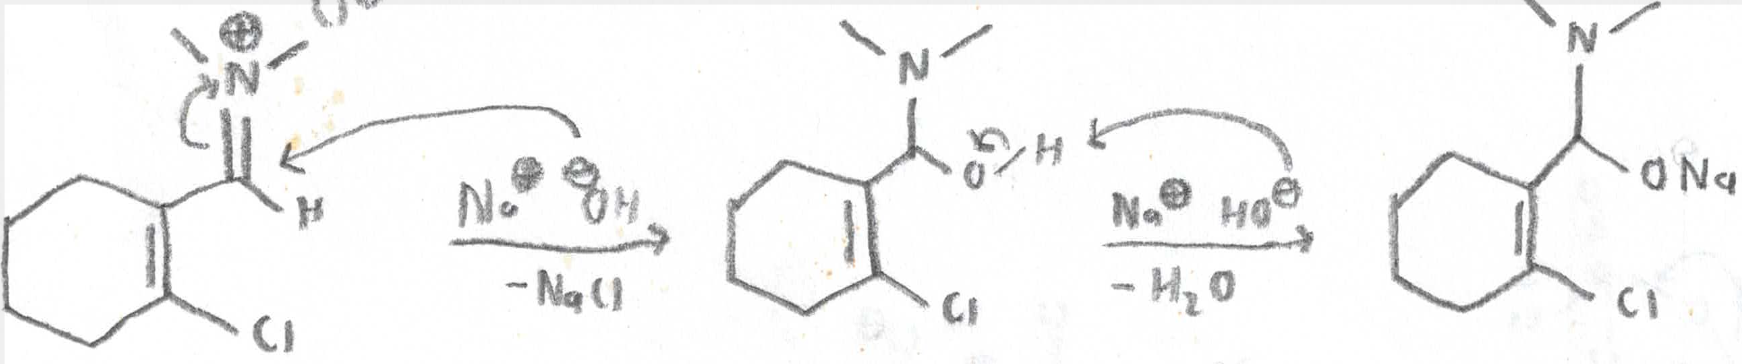
\includegraphics[width=0.6\linewidth]{VHClCHOMechd.png}
            \caption{Basic hydrolysis.}
            \label{fig:VHClCHOMechd}
        \end{subfigure}\\[2em]
        \begin{subfigure}[b]{\linewidth}
            \centering
            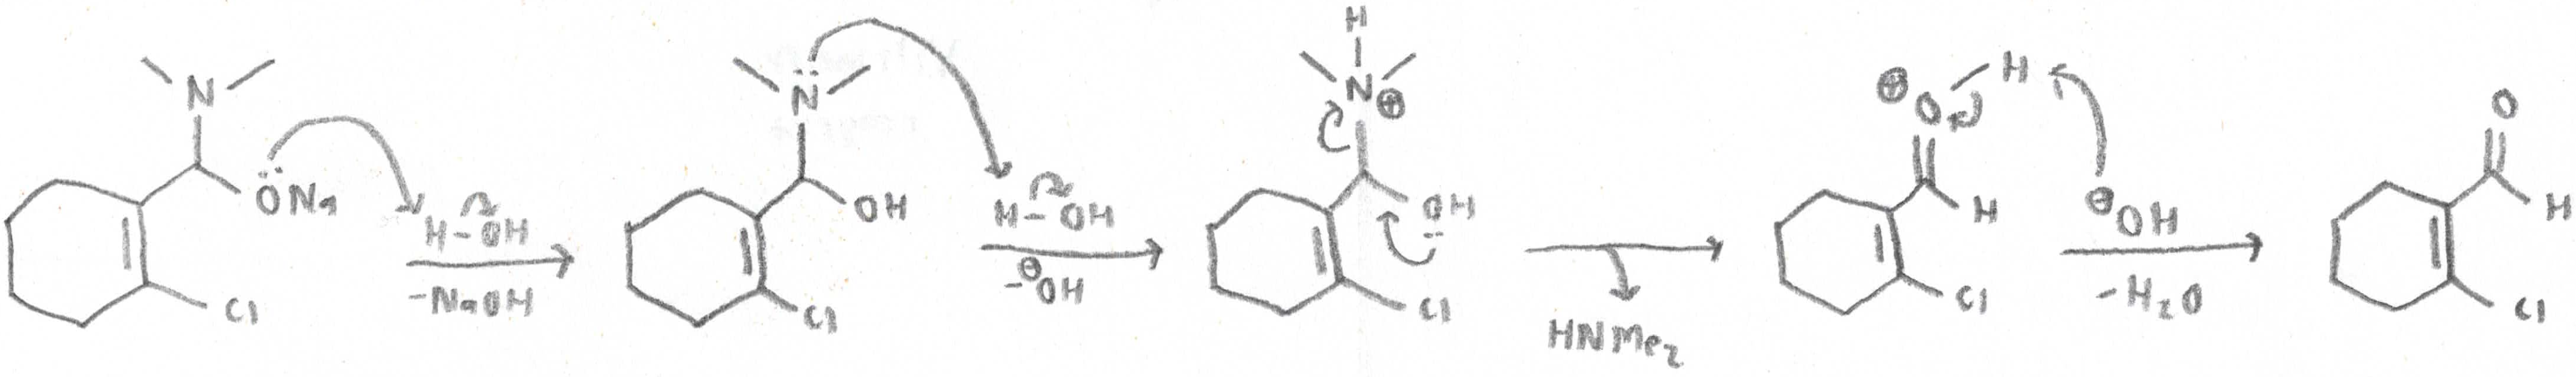
\includegraphics[width=0.85\linewidth]{VHClCHOMeche.png}
            \caption{Neutral/acidic hydrolysis.}
            \label{fig:VHClCHOMeche}
        \end{subfigure}
        \caption{Vilsmeier-Haack chloroformylation mechanism.}
        \label{fig:VHClCHOMech}
    \end{figure}
    \begin{itemize}
        \item \textbf{Vilsmeier reagent} prep (Figure \ref{fig:VHClCHOMecha}).
        \begin{itemize}
            \item To a solution of excess DMF, \ce{POCl3} is added. Thus, \ce{POCl3} will react completely with DMF to form the Vilsmeier reagent (and \ce{PO2Cl} byproduct). Said reagent will then be solubilized in the leftover DMF. This all occurs without competing reactivity with the ketone.
            \item Even if a ketone was present, \ce{POCl3} would prefer to react with DMF over the ketone because DMF's carbonyl is more reactive than the ketone's owing to the conjugated nitrogen lone pair.
            \item DMF also reacts exclusively through its oxygen instead of its nitrogen because its nitrogen is dialkylated, so it cannot undergo amide-iminol tautomerization.
        \end{itemize}
        \item Liberation of \ce{HCl} (Figure \ref{fig:VHClCHOMechb}).
        \begin{itemize}
            \item When the ketone is added to solution, very little of it (about one molecule in a million) will be in the reactive enol form. Thus, the element most susceptible to immediate electrophilic attack by the Vilsmeier reagent is the ketone's lone pairs.
            \begin{itemize}
                \item It is interesting that DMF does not attack the Vilsmeier reagent; or perhaps it only does so reversibly.
                \item Perhaps this reaction is unfavorable because the resulting iminium ion would have DMF as a much better leaving group (entropically and enthalpically in a polar aprotic solvent) then chloride.
            \end{itemize}
            \item Regardless, once the ketone attacks the Vilsmeier reagent, the resulting oxocarbenium ion's $\alpha$-protons are greatly activated toward deprotonation, perhaps by the chloride formerly of the Vilsmeier reagent salt. This leads to \ce{HCl} liberation.
            \item Now that there is no risk of forming an enthalpically unfavorable dication, the nitrogen lone pair is free to remove the chloride ion, reforming the more stable iminium salt (in a kind of no-bond resonance). The resultant species will not react further productively.
        \end{itemize}
        \item However, the damage is done, and the liberated \ce{HCl} can now catalyze the main sequence of steps.
        \item The main reaction (Figure \ref{fig:VHClCHOMechc}).
        \begin{itemize}
            \item \ce{HCl} has $\pKa=-6.3$, comparable to a protonated ketone's $-6$ to $-8$. Thus, \ce{HCl} can now easily protonate a ketone in solution, accelerating keto-enol tautomerization.
            \begin{itemize}
                \item \ce{HCl} could surely protonate many other species, too, but this is the only productive reactivity so it will predominantly control experimental results.
            \end{itemize}
            \item Keto-enol tautomerization yields an alkene that is sufficiently nucleophilic to attack another equivalent of the Vilsmeier reagent.
            \item The protonated ketone can then be deprotonated (liberating more \ce{HCl}), and an iminium chloride salt reformed.
            \item The $\beta$-ketoiminium chloride has a \emph{significantly} acidic $\alpha$-proton, and a base in solution (shown as chloride, for the sake of balancing everything) can deprotonate it to yield another equivalent of \ce{HCl}, as well as a conjugation-stabilized vinyligous amide.
            \begin{itemize}
                \item The increasing concentration of \ce{HCl} in solution results in an experimentally observable autocatalytic rate increase.
                \item It is important to remember that conjugated alkenes are more stable than unconjugated ones, hence why the vinyligous amide is more thermodynamically stable than the $\beta$-ketoiminium ion.
                \item This vinyligous amide intermediate can actually be isolated in some schemes!
            \end{itemize}
            \item We now want to get rid of the ketone oxygen. To do so, another equivalent of the Vilsmeier reagent will be used to turn it into a better leaving group. This leads to the formation of a labile (unstable) bisiminium chloride.
            \begin{itemize}
                \item Note that in much the same way that DMF's oxygen is activated toward nucleophilic attack by its nitrogen, the vinyligous amide's oxygen is activated by the further away, conjugated nitrogen.
            \end{itemize}
            \item Under the heated conditions of the reaction, the bisiminium chloride is subject to attack at the $\beta$-position of the conjugated iminium ion, followed by a collapse that kicks out DMF as a great leaving group (strong \ce{C=O} bond formation, amide-type conjugation, entropically favorable dissolution in the DMF solvent, etc.).
            \item We have now arrived at a species that is stable until workup.
        \end{itemize}
        \item In most procedures, basic workup appears to be a prerequisite to neutralization (Figure \ref{fig:VHClCHOMechd}).
        \item Then, under acidic or neutral conditions, we get the collapse to the aldehyde (Figure \ref{fig:VHClCHOMeche}).
        \begin{itemize}
            \item Note that this sequence of collapse to an aldehyde holding off until neutral or acidic conditions is reminiscient of Figure 3.7 in \textcite{bib:5-511Notes}.
            \item Indeed, under basic conditions, an anion is more stable on oxygen than nitrogen; but under acidic conditions, a nitrogen is more easily protonated (and hence used as a leaving group) than an oxygen.
        \end{itemize}
        \item It is worth noting that salt formation appears to be a driving force to be aware of, perhaps due to Coulombic attraction being more thermodynamically stable than covalent bond formation in some cases.
        \item References.
        \begin{itemize}
            \item \textcite[3663-3665]{bib:VilsmeierChloroformylationMech} --- review with currently accepted reaction mechanism outline.
            \item \textcite[12-13]{bib:VilsmeierChloroformylationPrep} --- standard prep for Vilsmeier-type chloroformylation.
        \end{itemize}
    \end{itemize}
    \item Now some older chemistry.
    \begin{itemize}
        \item Pyrimidines can be anti-asthma reagents.
        \item \textbf{Dimroth rearrangement} is quite interesting, but we don't have to know it (it's pretty esoteric).
    \end{itemize}
    \item Skipping Biginelli.
    \item Example synthesis: An $\alpha_1$-Adrenoceptor Antagonist.
    \begin{itemize}
        \item Useful reagent, \ce{POCl3}, S\textsubscript{N}Ar, deprotection.
        \item Aside: We should be saying in this class, "this again?!"
        \begin{itemize}
            \item Lots of condensations, S\textsubscript{N}Ar, dehydrations, etc.
        \end{itemize}
    \end{itemize}
    \item Example synthesis: GABA $\alpha 2/3$ agonist.
    \begin{itemize}
        \item Europe is on the move to ban all fluorine-containing drugs.
        \item But how do you make \ce{CF3}-containing compounds?
        \begin{itemize}
            \item \ce{CF3-} equivalents are really expensive to use on a large scale.
            \item Ideally, use TFA or anhydride; can also use \ce{CF3H}, but this is a greenhouse gas 500-2000 times worse than \ce{CO2}.
        \end{itemize}
        \item They use the anhydride; Friedel-Crafts type reaction with ethyl vinyl ether.
        \item Michael addition with guanidinium ion produces the core structure next.
        \item Next reagent is the synthetic equivalent of $\alpha$-bromoacetaldehyde.
    \end{itemize}
    \item Example (medchem) synthesis: DNA-dependent kinase inhibitor.
    \begin{itemize}
        \item Steve loves these compounds with high densities of nitrogens; this one has 8.
        \item Strategy: Break into smaller heterocycles and use \ce{C-N} cross-coupling.
        \item The first reagent is an amide acetal (specifically, the dimethyl acetal of DMF, analogous to \textbf{Brederech's reagent}). It makes nitrogen into an electrophile; you acylate this, and then get intramolecular S\textsubscript{N}2.
        \item ??, Curtius rearrangement, \ce{C-N} coupling with a Buchwald ligand (BrettPhos) on a palladium catalyst.
    \end{itemize}
    \item Example synthesis: Fungicidal compound.
    \begin{itemize}
        \item Key disconnection is a Suzuki-Miyaura cross-coupling.
        \item 2-iodo-5-bromopyridine isn't too hard to access. Then you make the 2-metallopyridine with \textbf{turbogrignard} (isopropyl magnesium chloride); negative charge attacks the halide (Br or I) to form the more stable anion.
        \item This anion attacks PivCl.
        \item Then lithiation and attack at the ketone.
        \item Other route: Sequential alkylation to form the cyclobutane, even in the presence of a fairly weak base.
        \item Then more turbogrignard (this time with the bromide) to generate the boronic acid. We can do this in the presence of a nitrile, presumably because the nitrile is so hindered.
    \end{itemize}
    \item We now move onto 5-membered heterocycles.
    \begin{itemize}
        \item Steve loves these, particular ones with multiple heteroatoms.
        \item Their reactions are typically more challenging, so most people avoid them. They're also of great interest in many applications.
    \end{itemize}
    \item \textbf{Pyrrole}. \emph{Etymology} from Greek "bright red color which pyrrole imparts to pinewood shavings moistened with concentrated hydrochloric acid."\footnote{Steve wonders, "How do you think to do that?!"}
    \begin{itemize}
        \item Most chemistry started in Germany, because they had a huge coal industry and most heterocycles were originally isolated from coal tar.
        \item PE and PP were invented (by accident) at the Max Planck institute, specifically the Ziegler-Natta polymerization; at Max Planck, they only call it the "Ziegler" polymerization.
        \item Pyrrole is $\pi$-excessive; it's more electron-rich. Unlike in pyridine, the nitrogen lone pair is \emph{part} of the aromatic system. This leads to anionic charges all throughout the ring.\footnote{If so electron rich, could help prevent thionolactonization tautomerization??}
        \item $\pKa$ of protonated pyrrole is $-3.8$, and the proton actually resides on carbon (because the pyrrole nitrogen is so nonbasic).
        \item Not quite as aromatic as benzene, but still pretty aromatic.
        \item Tetramethylpyrrole has $\pKa=3.7$ (methyl groups' hyperconjugation induces seven orders of magnitude difference). Also, now we protonate on the nitrogen (different in slides)??
    \end{itemize}
    \item Very susceptible to EAS.
    \begin{itemize}
        \item $\alpha$-position is slightly more active than $\beta$-position ($4:1$ ratio in nitration).
        \item So electrophilic that bromination (even under mild conditions) goes straight to tetrabrominated material.
        \item Monobromination can be accomplished with an alternative electrophilic bromine equivalent to NBS, called \textbf{dibromodimethylhydantoin}.
        \item Boc protection allows you to do mono- or di-$\alpha$-brominated pyrrole.
        \item TIPS protection allows you to do mono- or di-$\beta$-brominated pyrrole.
    \end{itemize}
    \item When you do something to the nitrogen, you do not disrupt aromaticity.
    \item \textbf{Vilsmeier} is classic; this is the best way to make 2-pyrrolylaldehydes.
    \item Electrocyclic reactions.
    \begin{itemize}
        \item Pyrrole is a very poor diene.
    \end{itemize}
    \item Decarboxylation can be nice; can be much easier to synthesize carboxylated than decarboxylated version.
    \item Cross-coupling reactivity of pyrrole.
    \begin{itemize}
        \item The choice of protecting group is key, and TIPS is usually best.
        \item Protecting group-dependent coupling applies to the Miyaura borylation and everything else.
    \end{itemize}
    \item Selected pyrrole syntheses.
    \begin{itemize}
        \item Classic disconnections give unstable precursors (esp. the dialdehyde), so we need synthetic equivalents.
        \item Pyrrole is no longer made from coal tar; it is today made commercially from furan.
        \begin{itemize}
            \item Alternative big synthesis: Pyrolyzing the sugar derivative, \textbf{ammonium mucate}. This is entropically very favorable.
        \end{itemize}
        \item Classic way for an organic or medicinal chemist to do this: \textbf{Paal-Knorr synthesis}.
        \begin{itemize}
            \item There are, in fact, lots of Knorr syntheses.
            \item The issue is that you can't buy that many 1,4-dicarbonyl compounds.
            \item Enamines (in mild acid) protonate at carbon (they protonate at nitrogen in strong acids). Pyrrole is essentially an enamine!
        \end{itemize}
        \item \textbf{Knorr} (pyrrole synthesis).
        \begin{itemize}
            \item $\alpha$-aminocarbonyl and $\beta$-ketoEWG (e.g., $\beta$-ketoester).
            \item Imine formation, followed by aldol-like condensation.
            \item Example: 2-aminoacetone and an activated system; activated because you don't want self-condensation.
            \item Saponify the methyl ester selectively, distill to remove \ce{CO2}.
            \item Write mechanisms for all transformations!!
        \end{itemize}
        \item \textbf{Hantzsch} (pyrrole synthesis).
        \begin{itemize}
            \item $\alpha$-halocarbonyl (no self-condensation!) and $\beta$-ketoEWG.
            \item Alkylation followed by ammonia.
            \item Example given.
        \end{itemize}
        \item \textbf{van Leusen} (pyrrole synthesis).
        \begin{itemize}
            \item More unusual.
            \item There are also several van Leusen syntheses of 5-membered heterocycles, all using TosMIC (an \textbf{isocyanide}, which is a type of heteroatom-stabilized carbene).
            \item Mechanism: After deprotonation of the acidic TosMIC $\alpha$-proton, Michael addition occurs. The resultant enolate adds at the isocyanide carbon to make the imino carbanion. Following protonation, the activated $\alpha$-proton of the $\beta$-iminoketone gets deprotonated, generating an electron conduit through wich to eject a tosyl leaving group. Finally, intramolecular proton transfer gives the desired pyrrole derivative.
            \item Compatible with HWE to introduce functional groups at C3 and C4 from an aldehyde and phosphonate ester.
        \end{itemize}
        \item Pyrrole is a great nitrogen protecting group; what else doesn't have a free NH? This is a quite common protecting group, even in Steve's collaboration with BMS.
    \end{itemize}
    \item Example synthesis: Remdesivir (COVID-19 drug).
    \begin{itemize}
        \item Required an efficient route to a certain heterocycle (on a 100 ton scale).
        \item Has to be done efficiently, cheaply, reliable, no bad waste stream, and SMs are basically "air, earth, fire, and water;" things you can get very cheaply from a variety of sources.
        \item Chlorosulfonylisocyanate is a quite old reagent. Installs a nitrile (good to draw mechanism!!). Then Pinner-type reagent.
        \item This was ok for the first few tons (33\% yield over 4 steps).
        \item Take pyrrole itself (write mechanism for Vilsmeier-type reaction!! Intermediacy of an oxime, followed by dehydration of the oxime).
        \item Then \ce{N-N} bond from chloramine.
        \item Two telescoped transformations increases yield by about 50\%!
    \end{itemize}
    \item Addendum: CSI-type nitrile installation.
    \begin{figure}[h!]
        \centering
        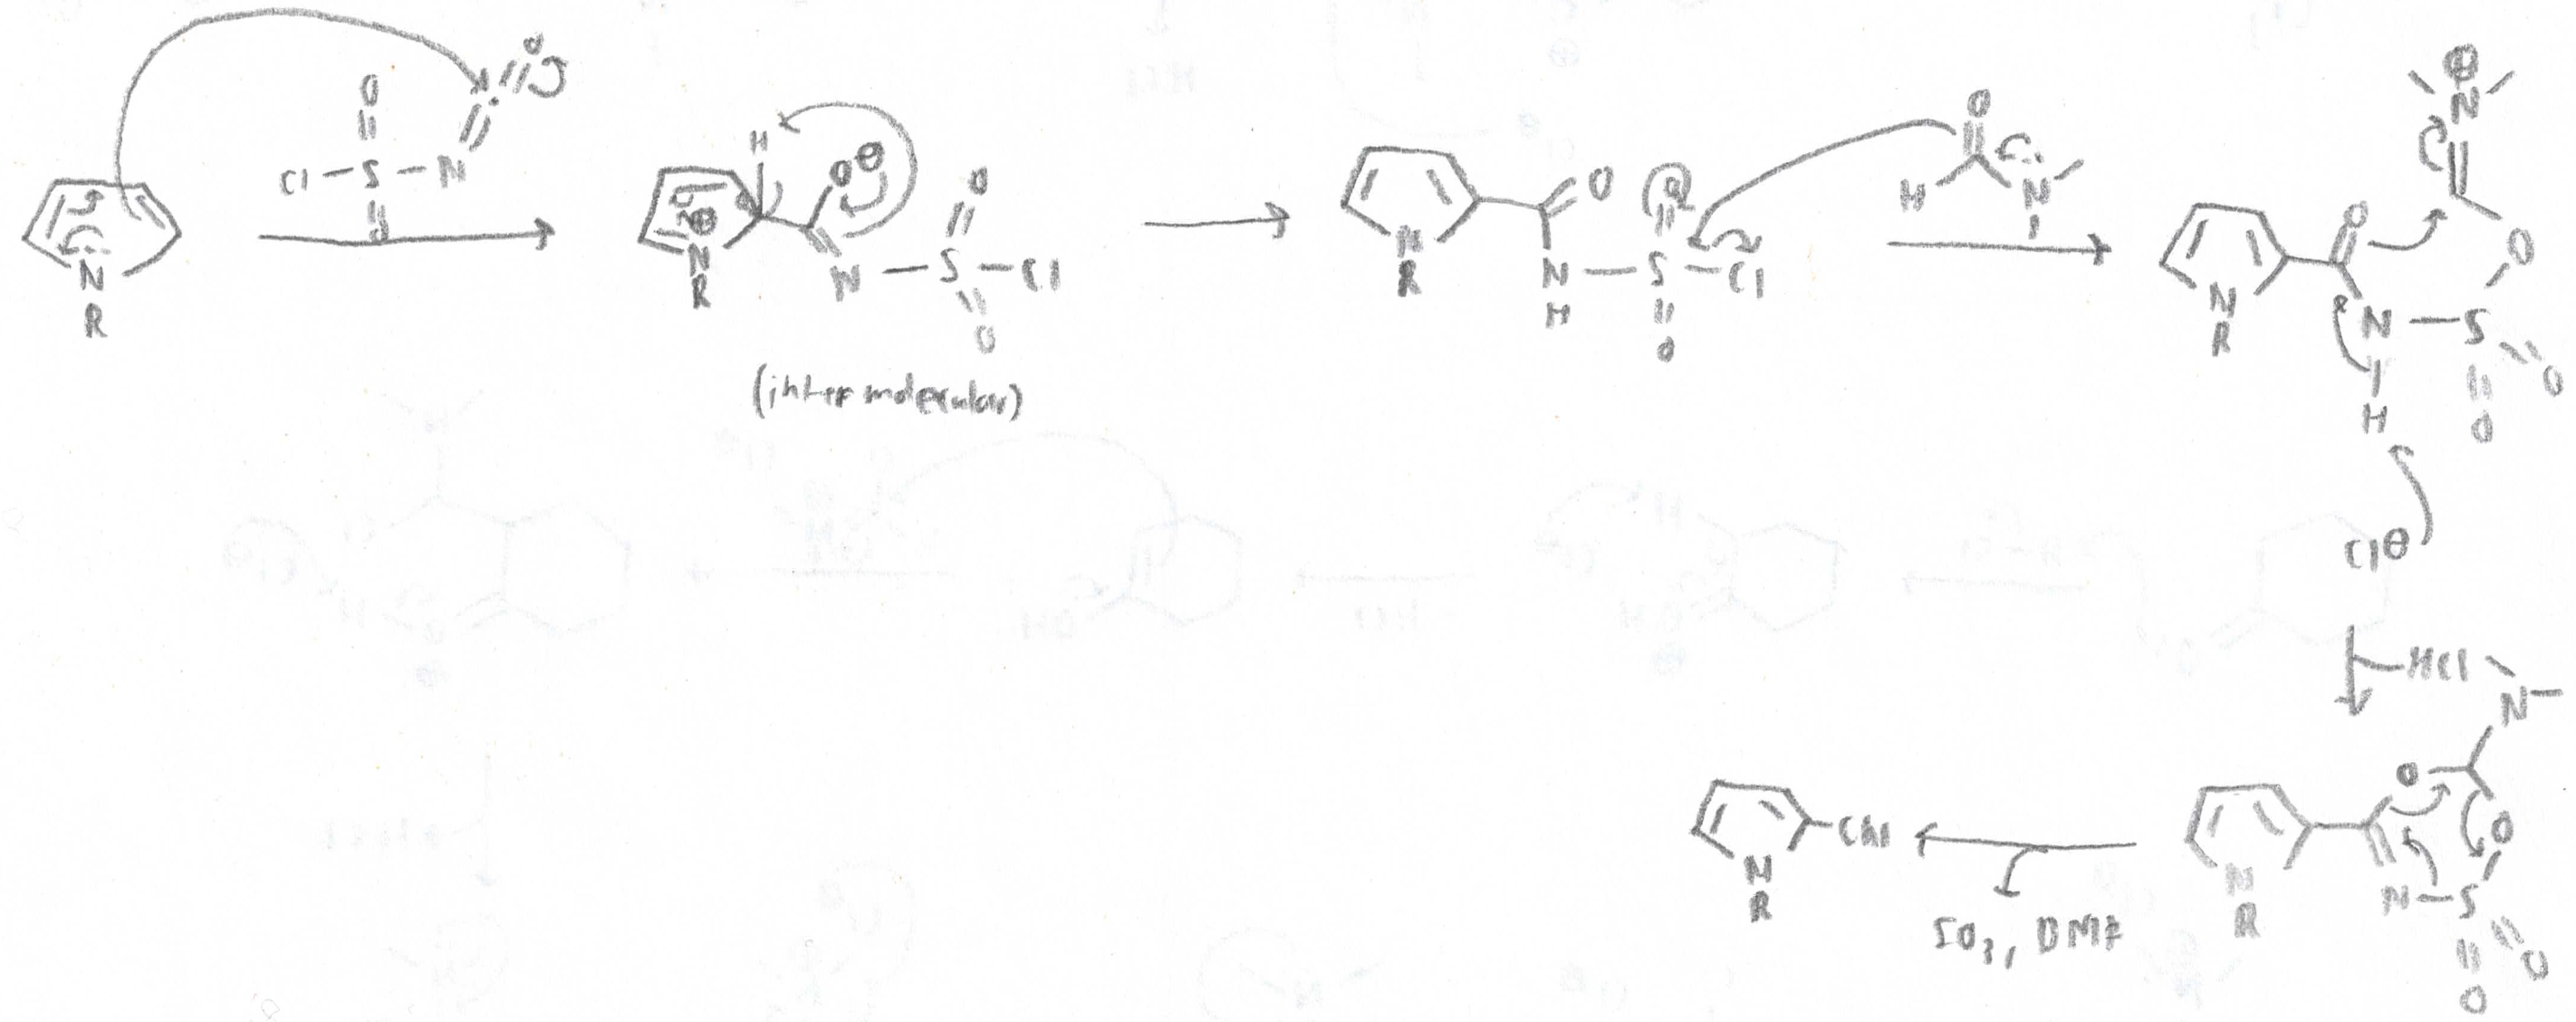
\includegraphics[width=0.85\linewidth]{CSI.png}
        \caption{Chlorosulfonylisocyanate-induced nitrile installation.}
        \label{fig:CSI}
    \end{figure}
    \begin{itemize}
        \item CSI's electrophilic isocyanate induces EAS-type reactivity from the nucleophilic pyrrole.
        \item Then PT occurs to the more nucleophilic isocyanate nitrogen (most likely intermolecular, contrary to how it's drawn). This also has rearomatization as a favorable driving force.
        \item At this point, we're pretty stable, but the solvent DMF can get involved. A few pericyclic reactions later, we get DMF back, strong \ce{S=O} bond formation in \ce{SO3}, \ce{HCl} catalyst formation, and our nitrile.
        \item Reference: \textcite[6553]{bib:CSI}.
    \end{itemize}
    \item \textbf{Volumetric productivity}: How much material can you get through your reactors in a given day? The better you do, the less the cost of your reactor dilutes the cost of your pharmaceutical.
    \begin{itemize}
        \item When you get to a certain scale, labor costs fall out of the equation.
    \end{itemize}
    \item Academics should spend less time on the cost and more time on the novelty of the chemistry.
    \item Six steps for a practical synthesis of the fluoro/ethyl ester.
    \begin{itemize}
        \item Aza-Michael addition.
        \item Protect nitrogen as Boc.
        \item Claisen to $\beta$-ketoester.
        \item Treatment with DAST (not particularly nice or cheap, but is effective).
        \item Pyrrolidine to dihydropyrrole, then a base as weak as \ce{Et3N} can form the shown product.
    \end{itemize}
    \item Lipitor.
    \begin{itemize}
        \item Largest-selling pharmaceutical (in terms of dollars) in the history of the world.
        \begin{itemize}
            \item Discovered at Park-Davis in Ann Arbor, a relatively small company. They partnered with Pfizer for the sales and marketing. They worked out a deal where they did well at low sales, but poorly at high sales; but this ended up being bad, and Pfizer acquired the company.
            \item Bruce Roth (the inventor) got laid off after 5 years, which kind of sucked.
        \end{itemize}
        \item Classic example of a statin.
        \begin{itemize}
            \item Along with penicillin antibiotics, statins changed the world more than almost any other pharmaceutical class.
        \end{itemize}
        \item Original synthesis: Paal-Knorr, enolate reduction, lactonization.
        \item $\beta$-ketoacids and esters are great substrates for asymmetric Noyori/Sharpless/Knowles chemistry.
        \item \textbf{Stetter} species reacts to form a carbon-carbon bond, then Michael addition.
        \item This material prepared from isoascorbic acid (available for 11 cents/gram).
    \end{itemize}
    \item Problem 3.
    \begin{figure}[h!]
        \centering
        \begin{subfigure}[b]{\linewidth}
            \centering
            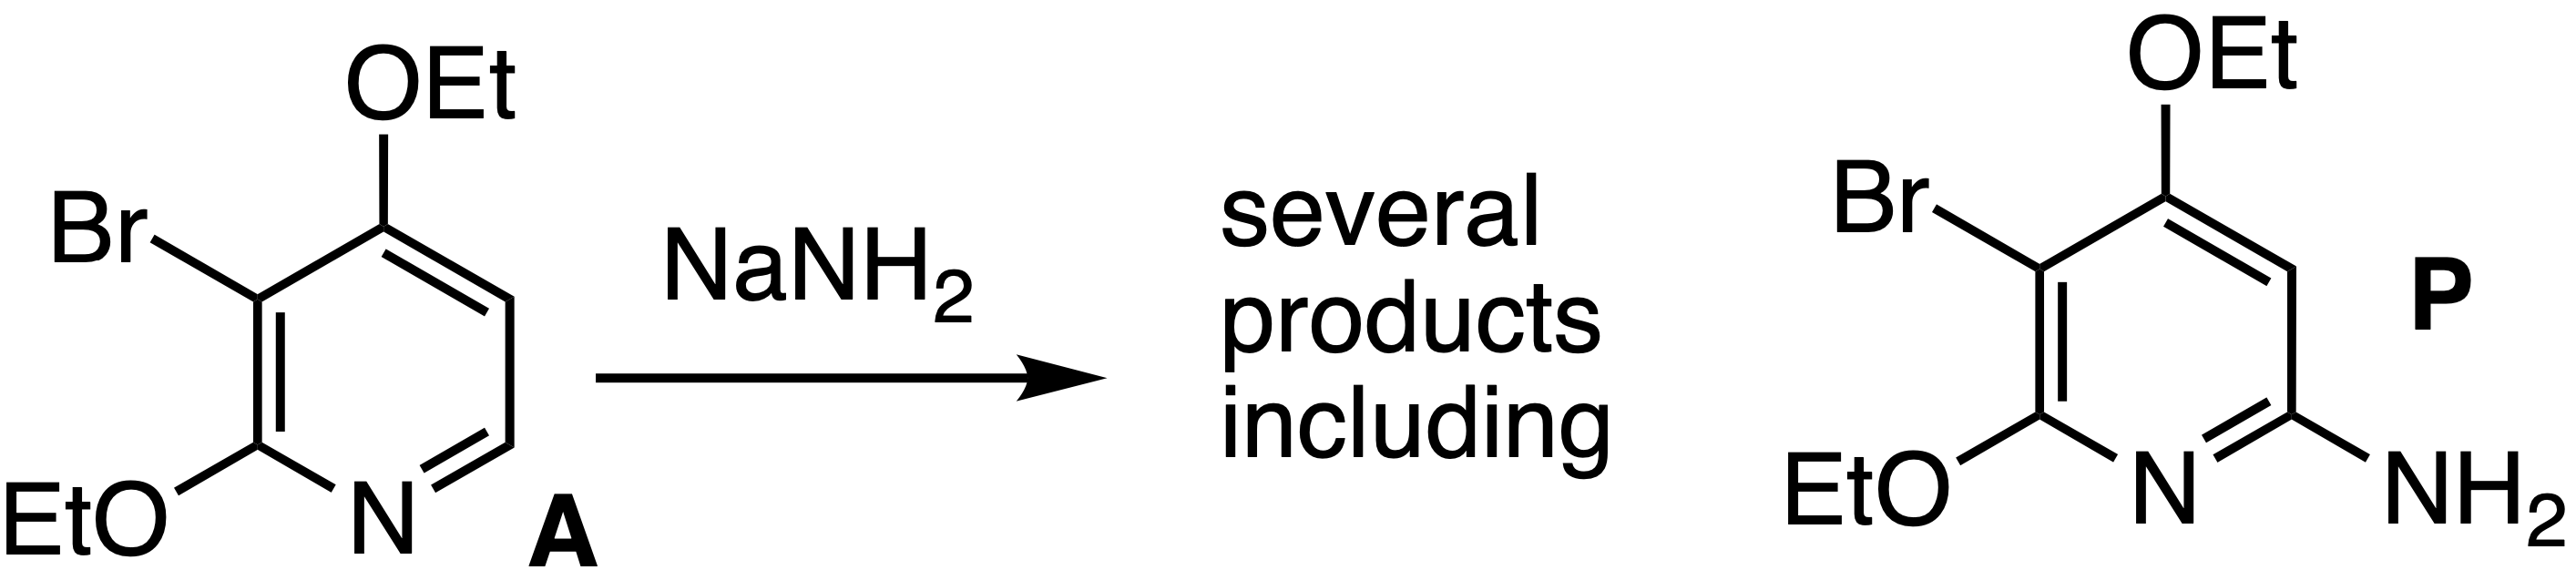
\includegraphics[width=0.45\linewidth]{TTQChichibabina.png}
            \caption{The reaction.}
            \label{fig:TTQChichibabina}
        \end{subfigure}\\[2em]
        \begin{subfigure}[b]{\linewidth}
            \centering
            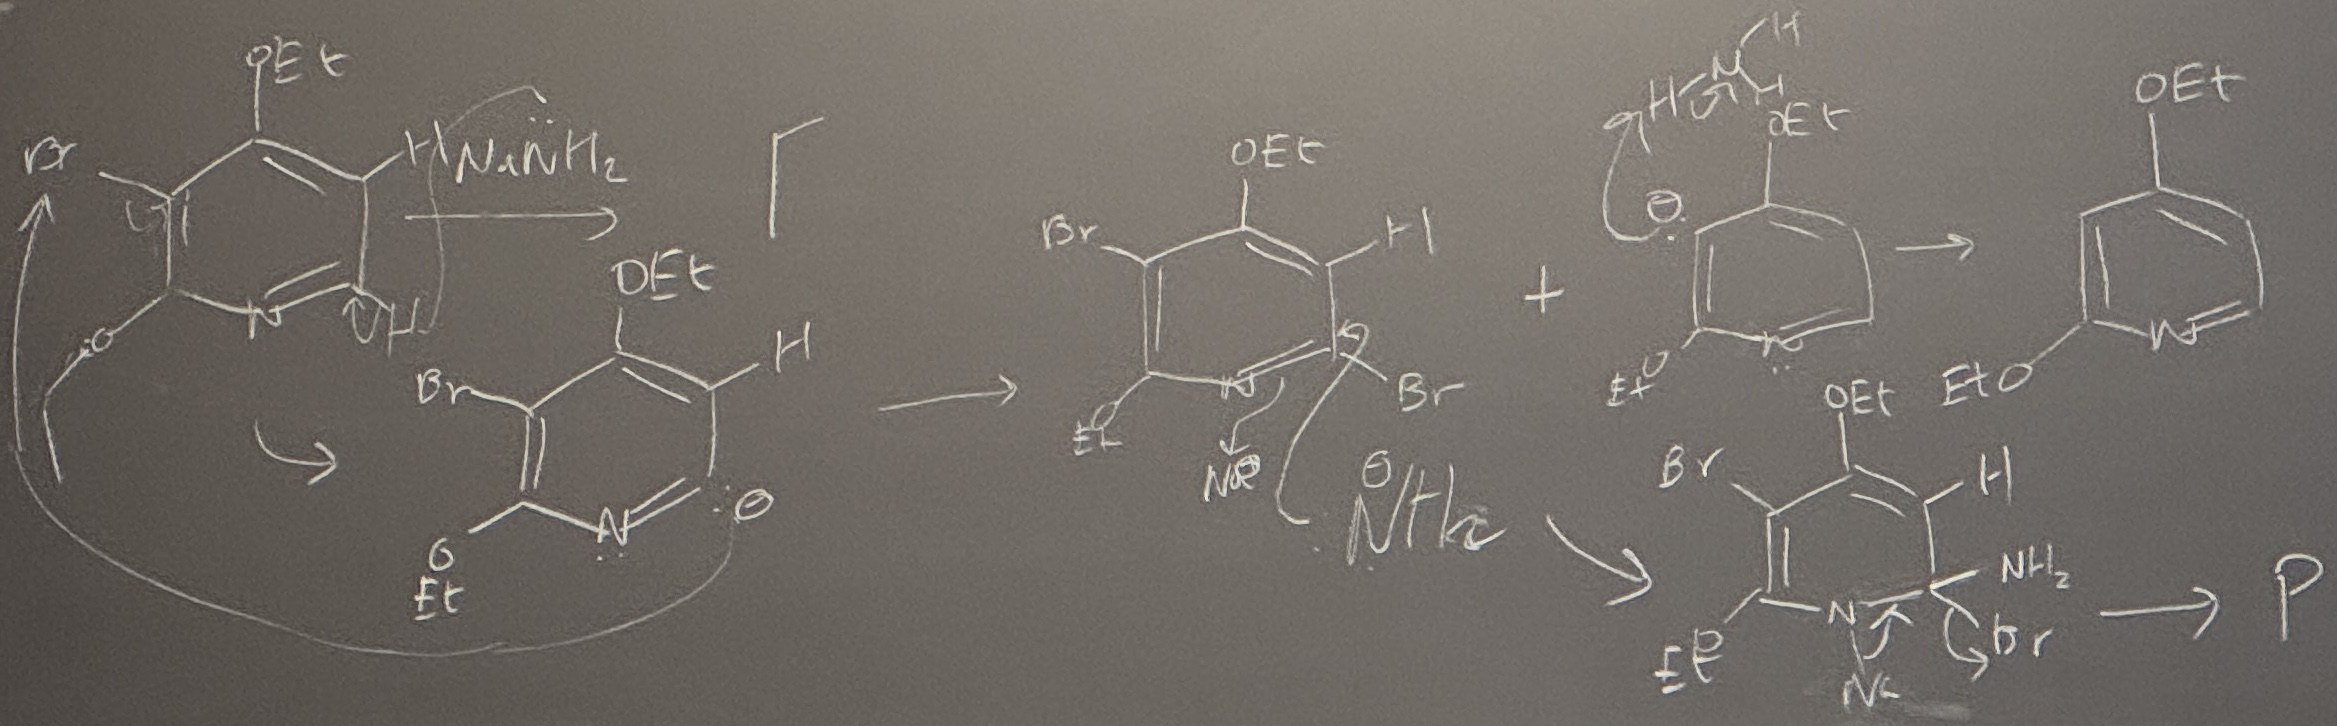
\includegraphics[width=0.7\linewidth]{TTQChichibabinb.JPG}
            \caption{A defensible mechanism.}
            \label{fig:TTQChichibabinb}
        \end{subfigure}\\[2em]
        \begin{subfigure}[b]{\linewidth}
            \centering
            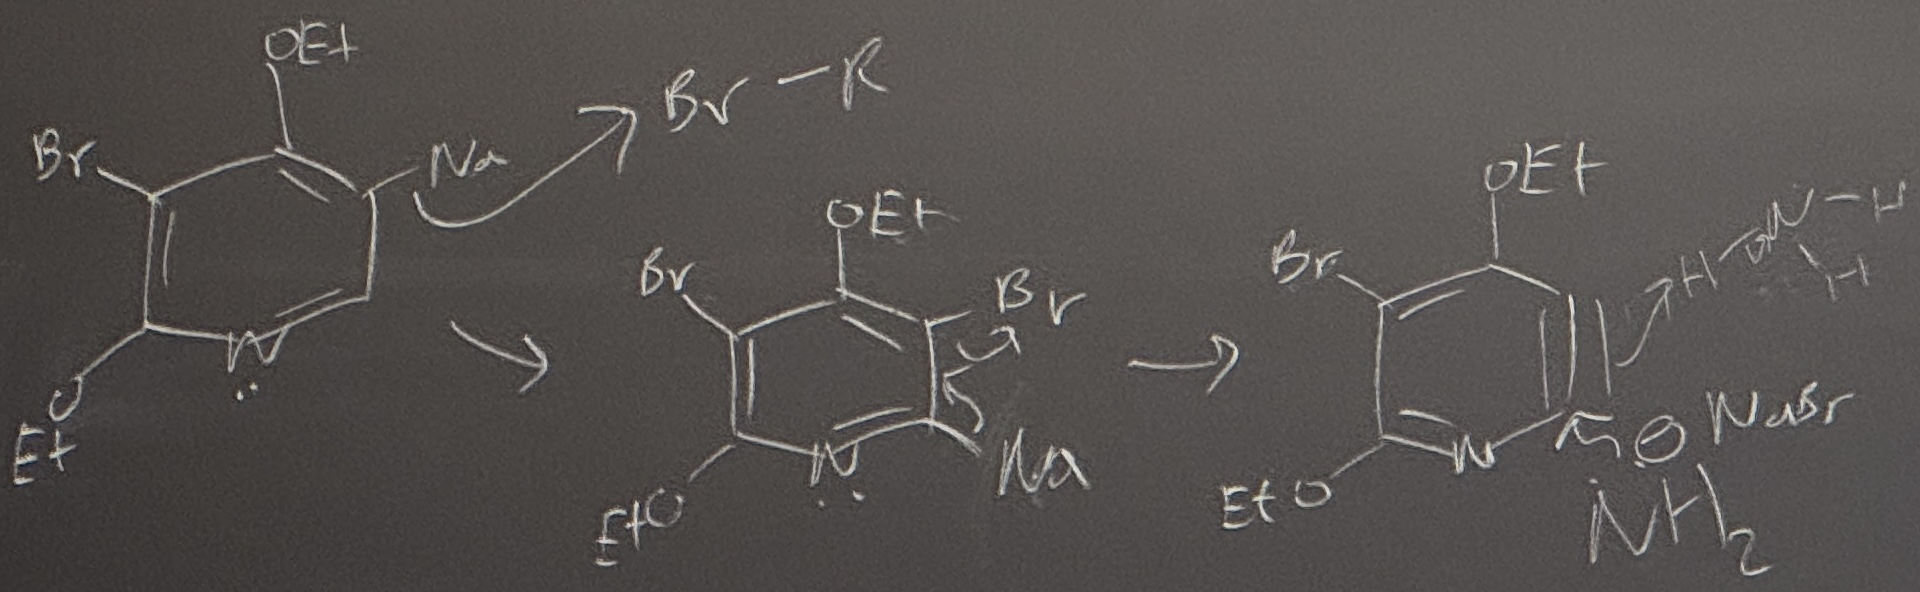
\includegraphics[width=0.55\linewidth]{TTQChichibabinc.JPG}
            \caption{Another defensible mechanism.}
            \label{fig:TTQChichibabinc}
        \end{subfigure}
        \caption{TTQ: Non-Chichibabin pyridine amination.}
        \label{fig:TTQChichibabin}
    \end{figure}
    \begin{itemize}
        \item \emph{Hint}: This reaction does \emph{not} proceed through a Chichibabin-type mechanism.
        \item Defensible mechanism 1 (Figure \ref{fig:TTQChichibabinb}).
        \begin{itemize}
            \item If we're not starting with addition chemistry, then let's start with abstraction/deprotonation chemistry!
            \begin{itemize}
                \item The \emph{meta}-position is usually more acidic in pyridines, but the alkoxides both add electron density to it. Thus, the \emph{ortho}-position is now more acidic.
                \item Deprotonating there gives an anion; now we have a species that \emph{cannot} be acted upon by a nucleophile.
            \end{itemize}
            \item Additionally, this anion is destabilized by the $\alpha$-effect.
            \begin{itemize}
                \item So, in the spirit of turbogrignard, we react at the bromide (through an ate complex) to form a new, more stable anion.
            \end{itemize}
            \item Then the new anion does intermolecular proton abstraction from the \ce{NH3} we produced.
            \item But now the 2-bromoposition is activated in the molecule that abstracted a bromide, so we can do a more classic Chichibabin with our better leaving group.
            \begin{itemize}
                \item Note that the second equivalent of \ce{NH2} attacks C2 instead of C5 because we can delocalize the C2 charge onto the nitrogen but not a hypothetical C5 charge.
            \end{itemize}
        \end{itemize}
        \item Follow-up question: What happens if we deprotonate at the other pyridine hydrogen position?
        \item Defensible mechanism 2 (Figure \ref{fig:TTQChichibabinc}).
        \begin{itemize}
            \item We start with the same type of bromine abstraction.
            \item This is followed by benzyne-type formation. We're under brutal conditions, so sodamide can act as a base again!
            \item From benzyne, the sodamide might attack it and then pick up a proton from the \ce{NH3}.
        \end{itemize}
        \item Differentiating the two mechanisms.
        \begin{itemize}
            \item KIEs could work.
            \item Selective deuteration of one position would also allow you to look at the product distribution and see whether the proton or deuteron got removed. In one, the deuteron will hang around; in the other, not.
        \end{itemize}
    \end{itemize}
\end{itemize}




\end{document}